\documentclass[]{book}
\usepackage{lmodern}
\usepackage{amssymb,amsmath}
\usepackage{ifxetex,ifluatex}
\usepackage{fixltx2e} % provides \textsubscript
\ifnum 0\ifxetex 1\fi\ifluatex 1\fi=0 % if pdftex
  \usepackage[T1]{fontenc}
  \usepackage[utf8]{inputenc}
\else % if luatex or xelatex
  \ifxetex
    \usepackage{mathspec}
  \else
    \usepackage{fontspec}
  \fi
  \defaultfontfeatures{Ligatures=TeX,Scale=MatchLowercase}
\fi
% use upquote if available, for straight quotes in verbatim environments
\IfFileExists{upquote.sty}{\usepackage{upquote}}{}
% use microtype if available
\IfFileExists{microtype.sty}{%
\usepackage{microtype}
\UseMicrotypeSet[protrusion]{basicmath} % disable protrusion for tt fonts
}{}
\usepackage{hyperref}
\hypersetup{unicode=true,
            pdftitle={mev package tutorial},
            pdfauthor={Léo Belzile},
            pdfborder={0 0 0},
            breaklinks=true}
\urlstyle{same}  % don't use monospace font for urls
\usepackage{natbib}
\bibliographystyle{apalike2}
\usepackage{color}
\usepackage{fancyvrb}
\newcommand{\VerbBar}{|}
\newcommand{\VERB}{\Verb[commandchars=\\\{\}]}
\DefineVerbatimEnvironment{Highlighting}{Verbatim}{commandchars=\\\{\}}
% Add ',fontsize=\small' for more characters per line
\usepackage{framed}
\definecolor{shadecolor}{RGB}{248,248,248}
\newenvironment{Shaded}{\begin{snugshade}}{\end{snugshade}}
\newcommand{\AlertTok}[1]{\textcolor[rgb]{0.94,0.16,0.16}{#1}}
\newcommand{\AnnotationTok}[1]{\textcolor[rgb]{0.56,0.35,0.01}{\textbf{\textit{#1}}}}
\newcommand{\AttributeTok}[1]{\textcolor[rgb]{0.77,0.63,0.00}{#1}}
\newcommand{\BaseNTok}[1]{\textcolor[rgb]{0.00,0.00,0.81}{#1}}
\newcommand{\BuiltInTok}[1]{#1}
\newcommand{\CharTok}[1]{\textcolor[rgb]{0.31,0.60,0.02}{#1}}
\newcommand{\CommentTok}[1]{\textcolor[rgb]{0.56,0.35,0.01}{\textit{#1}}}
\newcommand{\CommentVarTok}[1]{\textcolor[rgb]{0.56,0.35,0.01}{\textbf{\textit{#1}}}}
\newcommand{\ConstantTok}[1]{\textcolor[rgb]{0.00,0.00,0.00}{#1}}
\newcommand{\ControlFlowTok}[1]{\textcolor[rgb]{0.13,0.29,0.53}{\textbf{#1}}}
\newcommand{\DataTypeTok}[1]{\textcolor[rgb]{0.13,0.29,0.53}{#1}}
\newcommand{\DecValTok}[1]{\textcolor[rgb]{0.00,0.00,0.81}{#1}}
\newcommand{\DocumentationTok}[1]{\textcolor[rgb]{0.56,0.35,0.01}{\textbf{\textit{#1}}}}
\newcommand{\ErrorTok}[1]{\textcolor[rgb]{0.64,0.00,0.00}{\textbf{#1}}}
\newcommand{\ExtensionTok}[1]{#1}
\newcommand{\FloatTok}[1]{\textcolor[rgb]{0.00,0.00,0.81}{#1}}
\newcommand{\FunctionTok}[1]{\textcolor[rgb]{0.00,0.00,0.00}{#1}}
\newcommand{\ImportTok}[1]{#1}
\newcommand{\InformationTok}[1]{\textcolor[rgb]{0.56,0.35,0.01}{\textbf{\textit{#1}}}}
\newcommand{\KeywordTok}[1]{\textcolor[rgb]{0.13,0.29,0.53}{\textbf{#1}}}
\newcommand{\NormalTok}[1]{#1}
\newcommand{\OperatorTok}[1]{\textcolor[rgb]{0.81,0.36,0.00}{\textbf{#1}}}
\newcommand{\OtherTok}[1]{\textcolor[rgb]{0.56,0.35,0.01}{#1}}
\newcommand{\PreprocessorTok}[1]{\textcolor[rgb]{0.56,0.35,0.01}{\textit{#1}}}
\newcommand{\RegionMarkerTok}[1]{#1}
\newcommand{\SpecialCharTok}[1]{\textcolor[rgb]{0.00,0.00,0.00}{#1}}
\newcommand{\SpecialStringTok}[1]{\textcolor[rgb]{0.31,0.60,0.02}{#1}}
\newcommand{\StringTok}[1]{\textcolor[rgb]{0.31,0.60,0.02}{#1}}
\newcommand{\VariableTok}[1]{\textcolor[rgb]{0.00,0.00,0.00}{#1}}
\newcommand{\VerbatimStringTok}[1]{\textcolor[rgb]{0.31,0.60,0.02}{#1}}
\newcommand{\WarningTok}[1]{\textcolor[rgb]{0.56,0.35,0.01}{\textbf{\textit{#1}}}}
\usepackage{longtable,booktabs}
\usepackage{graphicx,grffile}
\makeatletter
\def\maxwidth{\ifdim\Gin@nat@width>\linewidth\linewidth\else\Gin@nat@width\fi}
\def\maxheight{\ifdim\Gin@nat@height>\textheight\textheight\else\Gin@nat@height\fi}
\makeatother
% Scale images if necessary, so that they will not overflow the page
% margins by default, and it is still possible to overwrite the defaults
% using explicit options in \includegraphics[width, height, ...]{}
\setkeys{Gin}{width=\maxwidth,height=\maxheight,keepaspectratio}
\IfFileExists{parskip.sty}{%
\usepackage{parskip}
}{% else
\setlength{\parindent}{0pt}
\setlength{\parskip}{6pt plus 2pt minus 1pt}
}
\setlength{\emergencystretch}{3em}  % prevent overfull lines
\providecommand{\tightlist}{%
  \setlength{\itemsep}{0pt}\setlength{\parskip}{0pt}}
\setcounter{secnumdepth}{5}
% Redefines (sub)paragraphs to behave more like sections
\ifx\paragraph\undefined\else
\let\oldparagraph\paragraph
\renewcommand{\paragraph}[1]{\oldparagraph{#1}\mbox{}}
\fi
\ifx\subparagraph\undefined\else
\let\oldsubparagraph\subparagraph
\renewcommand{\subparagraph}[1]{\oldsubparagraph{#1}\mbox{}}
\fi

%%% Use protect on footnotes to avoid problems with footnotes in titles
\let\rmarkdownfootnote\footnote%
\def\footnote{\protect\rmarkdownfootnote}

%%% Change title format to be more compact
\usepackage{titling}

% Create subtitle command for use in maketitle
\providecommand{\subtitle}[1]{
  \posttitle{
    \begin{center}\large#1\end{center}
    }
}

\setlength{\droptitle}{-2em}

  \title{\texttt{mev} package tutorial}
    \pretitle{\vspace{\droptitle}\centering\huge}
  \posttitle{\par}
    \author{Léo Belzile}
    \preauthor{\centering\large\emph}
  \postauthor{\par}
      \predate{\centering\large\emph}
  \postdate{\par}
    \date{2019-06-28}

\usepackage[mathscr]{eucal}
\DeclareMathAlphabet{\mathcrl}{U}{rsfs}{m}{n}
\usepackage{fourier}
\DeclareMathAlphabet{\mathcal}{OMS}{cmsy}{m}{n}
\usepackage{booktabs}
\usepackage{amsthm}
\makeatletter
\def\thm@space@setup{%
  \thm@preskip=8pt plus 2pt minus 4pt
  \thm@postskip=\thm@preskip
}
\makeatother

\usepackage{framed,color}
\definecolor{shadecolor}{RGB}{248,248,248}

\renewcommand{\textfraction}{0.05}
\renewcommand{\topfraction}{0.8}
\renewcommand{\bottomfraction}{0.8}
\renewcommand{\floatpagefraction}{0.75}

\let\oldhref\href
\renewcommand{\href}[2]{#2\footnote{\url{#1}}}

\ifxetex
  \usepackage{letltxmacro}
  \setlength{\XeTeXLinkMargin}{1pt}
  \LetLtxMacro\SavedIncludeGraphics\includegraphics
  \def\includegraphics#1#{% #1 catches optional stuff (star/opt. arg.)
    \IncludeGraphicsAux{#1}%
  }%
  \newcommand*{\IncludeGraphicsAux}[2]{%
    \XeTeXLinkBox{%
      \SavedIncludeGraphics#1{#2}%
    }%
  }%
\fi

\makeatletter
\newenvironment{kframe}{%
\medskip{}
\setlength{\fboxsep}{.8em}
 \def\at@end@of@kframe{}%
 \ifinner\ifhmode%
  \def\at@end@of@kframe{\end{minipage}}%
  \begin{minipage}{\columnwidth}%
 \fi\fi%
 \def\FrameCommand##1{\hskip\@totalleftmargin \hskip-\fboxsep
 \colorbox{shadecolor}{##1}\hskip-\fboxsep
     % There is no \\@totalrightmargin, so:
     \hskip-\linewidth \hskip-\@totalleftmargin \hskip\columnwidth}%
 \MakeFramed {\advance\hsize-\width
   \@totalleftmargin\z@ \linewidth\hsize
   \@setminipage}}%
 {\par\unskip\endMakeFramed%
 \at@end@of@kframe}
\makeatother

\makeatletter
\@ifundefined{Shaded}{
}{\renewenvironment{Shaded}{\begin{kframe}}{\end{kframe}}}
\makeatother

\newenvironment{rmdblock}[1]
  {
  \begin{itemize}
  \renewcommand{\labelitemi}{
    \raisebox{-.7\height}[0pt][0pt]{
      {\setkeys{Gin}{width=3em,keepaspectratio}\includegraphics{images/#1}}
    }
  }
  \setlength{\fboxsep}{1em}
  \begin{kframe}
  \item
  }
  {
  \end{kframe}
  \end{itemize}
  }
\newenvironment{rmdnote}
  {\begin{rmdblock}{note}}
  {\end{rmdblock}}
\newenvironment{rmdcaution}
  {\begin{rmdblock}{caution}}
  {\end{rmdblock}}
\newenvironment{rmdimportant}
  {\begin{rmdblock}{important}}
  {\end{rmdblock}}
\newenvironment{rmdtip}
  {\begin{rmdblock}{tip}}
  {\end{rmdblock}}
\newenvironment{rmdwarning}
  {\begin{rmdblock}{warning}}
  {\end{rmdblock}}

\begin{document}
\maketitle

{
\setcounter{tocdepth}{1}
\tableofcontents
}
\hypertarget{preliminary-remarks}{%
\chapter*{Preliminary remarks}\label{preliminary-remarks}}
\addcontentsline{toc}{chapter}{Preliminary remarks}

The \texttt{mev} package bundles routine for
- likelihood-based inference for univariate extremes (including distributions, densities, score, information matrix and higher order asymptotics). The four basic likelihood (generalized extreme value, generalized Pareto, non-homogeneous Poisson process and \(r\)-largest) are implemented. For the first two distributions, additional higher order inference tools are available, including profile likelihoods in most parametrizations of interest. Many recent threshold selection diagnostics that have appeared in the literature are implemented.

The second includes multivariate goodness-of-fit diagnostics and tests (max-stability test, information matrix test, coefficient of tail dependence, extremal coefficient, estimators of the extremal index, extremogram, nonparametric estimation of the angular measure, etc.) Pairwise composite likelihood for general models will be included in a future update.

Last, but not least, the package includes functions to simulate from multivariate max-stable vectors in dimension \(d\geq 2\), including extensions of most of the families in the \texttt{evd} package. The package also includes simulation algorithms for \(R\)-Pareto processes using accept-reject and composition sampling, and accept-reject for generalized \(R\)-Pareto processes.

You can install the latest version of the package (\texttt{v.1.12}) directly from CRAN via

\begin{Shaded}
\begin{Highlighting}[]
\KeywordTok{install.packages}\NormalTok{(}\StringTok{"mev"}\NormalTok{)}
\end{Highlighting}
\end{Shaded}

\newcommand{\bs}[1]{\boldsymbol{#1}}
\newcommand{\Hmat}{\mathbf{H}}
\newcommand{\Mmat}{\mathbf{M}}
\newcommand{\mX}{\mathbf{X}}
\newcommand{\bX}{{\mathbf{X}}}
\newcommand{\bx}{{\mathbf{x}}}
\newcommand{\by}{{\boldsymbol{y}}}
\newcommand{\bY}{{\boldsymbol{Y}}}
\newcommand{\eps}{\varepsilon}
\newcommand{\beps}{\boldsymbol{\varepsilon}}
\newcommand{\bbeta}{\boldsymbol{\beta}}
\newcommand{\hbb}{\hat{\boldsymbol{\beta}}}
\newcommand{\limni}{\lim_{n \ra \infty}}
\newcommand{\Sp}{\mathscr{S}}
\newcommand{\E}[2][]{{\mathsf E}_{#1}\left(#2\right)}
\newcommand{\Va}[2][]{{\mathsf{Var}_{#1}}\left(#2\right)}
\newcommand{\I}[1]{{\mathbf 1}_{#1}}
\newcommand{\R}{\mathbb{R}}
\newcommand{\N}{\mathbb{N}}
\newcommand{\Cn}{\textsf{No}}
\newcommand{\simiid}{\stackrel{\mathrm{iid}}{\sim}}
\newcommand{\bigO}{\mathrm{O}}
\newcommand{\rp}{\mathrm{p}}

\hypertarget{univariate-peaks-over-threshold-analysis}{%
\chapter{Univariate peaks-over-threshold analysis}\label{univariate-peaks-over-threshold-analysis}}

Let \(\ell(\boldsymbol{y}; \boldsymbol{\theta})\) denotes the log-likelihood of an \(n\) sample with a \(p\)-dimensional parameter \(\boldsymbol{\theta}\). The score vector is \(U(\boldsymbol{\theta})=\partial \ell / \partial \boldsymbol{\theta}\), while the Fisher information is \(i(\boldsymbol{\theta})=\mathrm{E}\{U(\boldsymbol{\theta})U(\boldsymbol{\theta})^\top\}\). Under regularity conditions, we also have \(i(\boldsymbol{\theta}) = - \mathrm{E}(\partial^2 \ell / \partial \boldsymbol{\theta}\partial \boldsymbol{\theta}^\top)\). The observed information is the Hessian \(-\partial^2 \ell / \partial \boldsymbol{\theta}\partial \boldsymbol{\theta}^\top\), evaluated at the maximum likelihood estimator \(\hat{\boldsymbol{\theta}}\).

By definition, the maximum likelihood estimator solves the score equation, i.e.~\(U(\hat{\boldsymbol{\theta}})=\boldsymbol{0}_p\). If the maximum likelihood estimator is not available in closed-form, this can be used to verify that the optimization routine has converged. It can also be used for Newton methods.

There are four basic likelihoods for univariate extremes: the likelihood of the generalized extreme value (GEV) distribution for block maxima, the likelihood for the generalized Pareto distribution and that of the non-homogeneous Poisson process (NHPP) for exceedances above a threshold \(u\), the likelihood of the \(r\)-largest observations, which can be used to model the \(r\)-largest observations per block or threshold exceedances where the threshold is the \(r\)th order statistic. The NHPP likelihood includes a contribution for the fraction of points that exceeds the threshold, whereas the generalized Pareto is a conditional distribution, whose normalizing constant \(\zeta_u=\Pr(Y>u)\) is the third parameter.

The generalized extreme value (GEV) distribution with location parameter \(\mu \in \mathbb{R}\), scale parameter \(\sigma \in \mathbb{R}_{+}\) and shape
parameter \(\xi \in \mathbb{R}\) is
\begin{align*}
  G(x)  = 
\begin{cases}
\exp\left\{-\left(1+\xi \frac{x-\mu}{\sigma}\right)^{-1/\xi}\right\}, &  \xi \neq 0,\\
\exp \left\{ -\exp \left(-\frac{x-\mu}{\sigma}\right)\right\},&  \xi = 0,
\end{cases} 
 \end{align*}
defined on \(\{x \in \mathbb{R}: \xi(x-\mu)/\sigma > -1\}\) where \(x_{+} = \max\{0, x\}\). The case \(\xi=0\) is commonly known as the Gumbel
distribution.
We denote the distribution by \(\mathsf{GEV}(\mu, \sigma, \xi)\).
\textbackslash end\{defn\}

The generalized Pareto (GP) distribution with scale \(\sigma \in \mathbb{R}_{+}\) and shape \(\xi \in \mathbb{R}\) is
\begin{align*}
  G(x)  = 
\begin{cases}
1-\left(1+\xi \frac{x}{\sigma}\right)_{+}^{-1/\xi}, &  \xi \neq 0,\\ 1-
\exp \left(-\frac{x}{\sigma}\right),&  \xi = 0.
\end{cases}
 \end{align*}
The range of the generalized Pareto distribution is \([0, -\sigma/\xi)\) if \(\xi < 0\) and is \(\mathbb{R}_{+}\) otherwise. We denote the distribution
by \(\mathsf{GP}(\sigma, \xi)\).

Let \(Y_{(1)} \geq \cdots \geq Y_{(r)}\) denote the \(r\) largest observations from a sample. The likelihood of the limiting distribution of the point process for the \(r\)-largest observations is \[
\ell(\mu,\sigma,\xi; \boldsymbol{y}) \equiv  -r\log(\sigma) - \left(1+\frac{1}{\xi}\right)\sum_{j=1}^r \log\left(1 + \xi\frac{y_{(j)}-\mu}{\sigma}\right)_{+} - \left(1 + \xi\frac{y_{(r)}-\mu}{\sigma}\right)^{-1/\xi}_+, \quad \mu,\xi\in\mathbb{R}, \sigma>0.
\]

Consider a sample of \(N\) observations, of which \(n_u\) exceed \(u\) and which we denote by \(y_1, \ldots, y_{n_u}\). The likelihood associated to the limiting distribution of threshold exceedances is
\begin{align}
L(\mu, \sigma, \xi; \boldsymbol{y}) = \exp \left[ - c \left\{1+ \xi \left( \frac{u-\mu}{\sigma}\right)\right\}^{-1/\xi}_{+}\right] (c\sigma)^{-n_u}\prod_{i=1}^{n_u} \left\{1+\xi\left( \frac{y_i-\mu}{\sigma}\right)\right\}^{-1/\xi-1}_{+}, \qquad \mu, \xi \in \mathbb{R}, \sigma >0, \label{eq:ppp_lik}
\end{align}
where \((\cdot)_{+} = \max\{0, \cdot\}\). The quantity \(c\) is a tuning parameter whose role is described in \S 7.5 of \citet{Coles:2001}. If we take \(c=N/m\), the parameters of the point process likelihood correspond to those of the generalized extreme value distribution fitted to blocks of size \(m\).

\hypertarget{profile-likelihood}{%
\subsection{Profile likelihood}\label{profile-likelihood}}

The profile
likelihood \(\ell_\mathrm{p}\), a function of \(\boldsymbol{\psi}\) alone, is obtained by maximizing the
likelihood pointwise at each fixed value \(\boldsymbol{\psi}=\boldsymbol{\psi}_0\) over the nuisance vector
\(\boldsymbol{\lambda}_{\psi_0}\),
\begin{align*}
   \ell_\mathrm{p}(\boldsymbol{\psi})=\max_{\boldsymbol{\lambda}}\ell(\boldsymbol{\psi}, \boldsymbol{\lambda})=\ell(\boldsymbol{\psi}, \hat{\boldsymbol{\lambda}}_{\boldsymbol{\psi}}).
\end{align*}
The observed profile information function is \index{information!observed (profile)}
\[j_\mathrm{p}(\boldsymbol{\psi})
=-\frac{\partial \ell_\mathrm{p}(\boldsymbol{\psi})}{\partial \boldsymbol{\psi}\partial \boldsymbol{\psi}^\top} 
= \left\{j^{\boldsymbol{\psi\psi}}(\boldsymbol{\psi}, \hat{\boldsymbol{\lambda}}_{\boldsymbol{\psi}})\right\}^{-1}.
\]
The profile likelihood is not a
genuine likelihood in the sense that it is not based on the density of a random variable.

This example illustrates some of the functions used in peaks-over-threshold analysis based on fitting a generalized Pareto distribution to threshold exceedances. We use the Venezuelian rainfall data, a time series of daily rainfall precipitations at Maiquetia airport in Venezuela, for the purpose of illustration.

\begin{Shaded}
\begin{Highlighting}[]
\KeywordTok{library}\NormalTok{(mev)}
\KeywordTok{library}\NormalTok{(lubridate, }\DataTypeTok{quietly =} \OtherTok{TRUE}\NormalTok{, }\DataTypeTok{warn.conflicts =} \OtherTok{FALSE}\NormalTok{)}

\KeywordTok{data}\NormalTok{(}\StringTok{"maiquetia"}\NormalTok{)}
\NormalTok{day <-}\StringTok{ }\KeywordTok{seq.Date}\NormalTok{(}\DataTypeTok{from =} \KeywordTok{as.Date}\NormalTok{(}\StringTok{"1961-01-01"}\NormalTok{), }
                \DataTypeTok{to =} \KeywordTok{as.Date}\NormalTok{(}\StringTok{"1999-12-31"}\NormalTok{), }\DataTypeTok{by =} \StringTok{"day"}\NormalTok{)}
\CommentTok{# Keep non-zero rainfall, exclude 1999 observations}
\NormalTok{nzrain <-}\StringTok{ }\NormalTok{maiquetia[}\KeywordTok{year}\NormalTok{(day) }\OperatorTok{<}\StringTok{ }\DecValTok{1999} \OperatorTok{&}\StringTok{ }\NormalTok{maiquetia }\OperatorTok{>}\StringTok{ }\DecValTok{0}\NormalTok{]}
\end{Highlighting}
\end{Shaded}

We will ignore temporal dependence and stationarity, but these should be considered.
The first step in our analysis is to choose a threshold. We select candidates based on quantiles and test whether they lead to stable inference.

\begin{Shaded}
\begin{Highlighting}[]
\NormalTok{ths <-}\StringTok{ }\KeywordTok{quantile}\NormalTok{(nzrain, }\KeywordTok{seq}\NormalTok{(}\FloatTok{0.9}\NormalTok{, }\FloatTok{0.99}\NormalTok{, }\DataTypeTok{length.out =} \DecValTok{15}\NormalTok{))}
\CommentTok{# Threshold selection diagnostics}
\KeywordTok{W.diag}\NormalTok{(}\DataTypeTok{xdat =}\NormalTok{ nzrain, }\DataTypeTok{model =} \StringTok{"nhpp"}\NormalTok{, }\DataTypeTok{plots =} \KeywordTok{c}\NormalTok{(}\StringTok{"WN"}\NormalTok{,}\StringTok{"PS"}\NormalTok{), }\DataTypeTok{u =}\NormalTok{ ths)}
\end{Highlighting}
\end{Shaded}

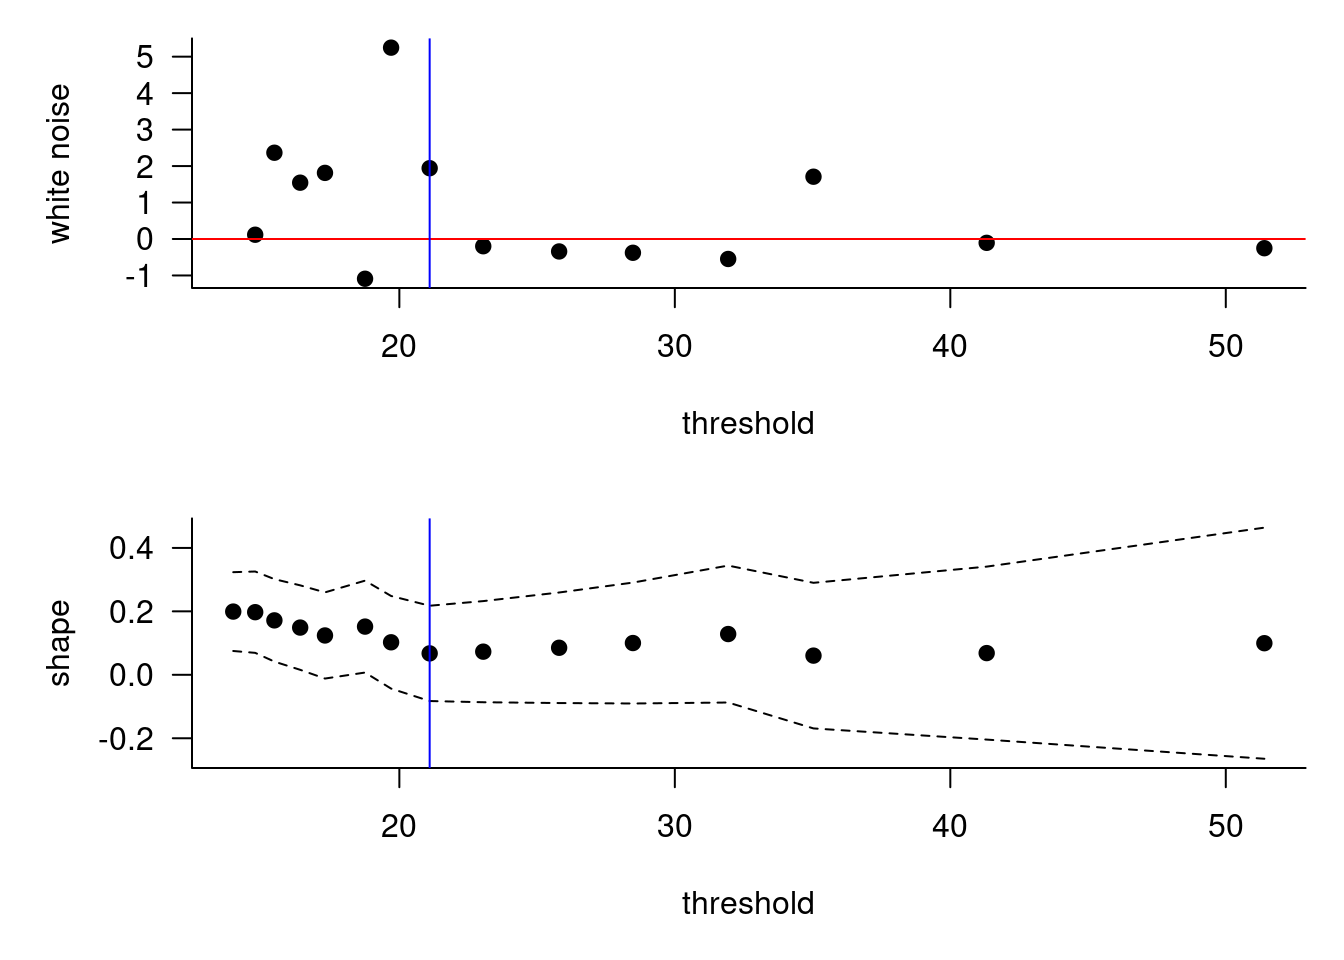
\includegraphics{mevtuto_files/figure-latex/unnamed-chunk-2-1.pdf}

\begin{Shaded}
\begin{Highlighting}[]
\KeywordTok{NC.diag}\NormalTok{(nzrain, }\DataTypeTok{u =}\NormalTok{ ths)}
\end{Highlighting}
\end{Shaded}

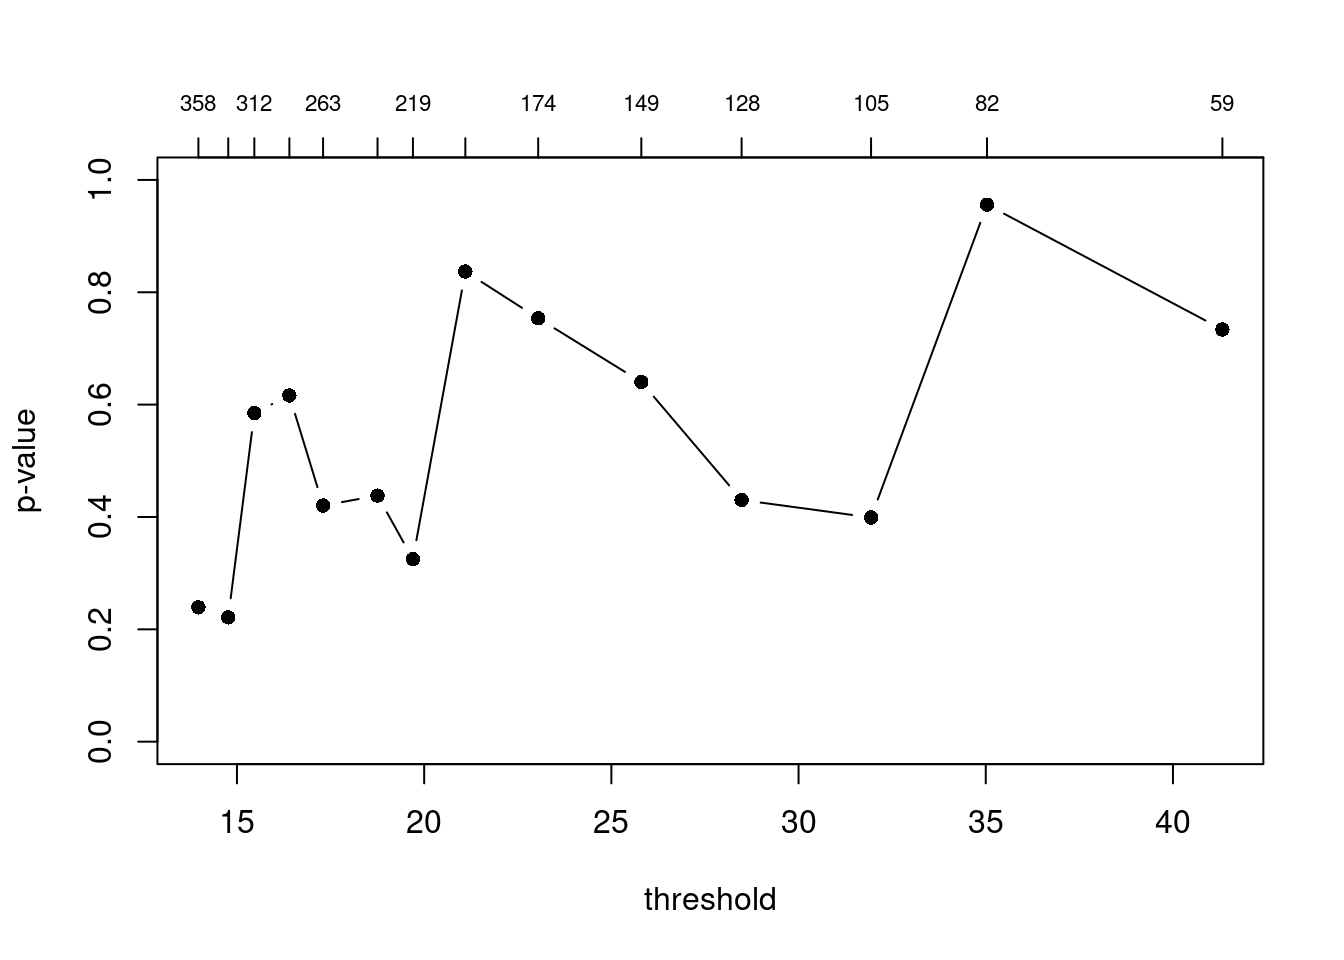
\includegraphics{mevtuto_files/figure-latex/unnamed-chunk-2-2.pdf}

Threshold selection diagnostics indicate that the shape is more or less constant over the range of threshold considered. Wadsworth's white noise sequence yields a very large residual around \(u=20\), but the Northrop--Coleman score test yields \(P\)-value path above 0.2 for every threshold under consideration.

\begin{Shaded}
\begin{Highlighting}[]
\CommentTok{# Fit using maximum likelihood estimation}
\NormalTok{gpdf <-}\StringTok{ }\KeywordTok{fit.gpd}\NormalTok{(nzrain, }\DataTypeTok{threshold =} \DecValTok{20}\NormalTok{, }\DataTypeTok{show =} \OtherTok{TRUE}\NormalTok{)}
\end{Highlighting}
\end{Shaded}

\begin{verbatim}
## Method: Grimshaw 
## Log-likelihood: -832.629 
## 
## Threshold: 20 
## Number Above: 216 
## Proportion Above: 0.0604 
## 
## Estimates
##   scale    shape  
## 15.5800   0.1088  
## 
## Standard Errors
##   scale    shape  
## 1.60673  0.07785  
## 
## Optimization Information
##   Convergence: successful
\end{verbatim}

The default optimization routine for the generalized Pareto distribution is
Grimshaw's method, which profiles out the likelihood. The method is almost guaranteed to converge. Because of non-regularity, the maximum likelihood estimator for \(\xi < -1\) does not solve the score equation and leads to infinite log-likelihood, hence the maximum returned lies on the boundary. The standard errors are based on the inverse observed information matrix and provided only if \(\xi>-1/2\). We can verify that our maximum likelihood estimate is indeed a maximum by checking if it solves the score equation if \(\hat{\xi}>-1\).

\begin{Shaded}
\begin{Highlighting}[]
\KeywordTok{isTRUE}\NormalTok{(}\KeywordTok{all.equal}\NormalTok{(}
  \KeywordTok{gpd.score}\NormalTok{(gpdf}\OperatorTok{$}\NormalTok{estimate, }\DataTypeTok{dat =}\NormalTok{ gpdf}\OperatorTok{$}\NormalTok{exceedances),}
  \KeywordTok{c}\NormalTok{(}\DecValTok{0}\NormalTok{,}\DecValTok{0}\NormalTok{), }\DataTypeTok{tolerance =} \FloatTok{1e-5}\NormalTok{))}
\end{Highlighting}
\end{Shaded}

\begin{verbatim}
## [1] TRUE
\end{verbatim}

If the sample is small, maximum likelihood estimators are biased for the generalized Pareto distribution (the shape parameter is negatively biased, regardless of the true value for \(\xi\)). Bias correction methods includes the modified score of Firth, but the default method is the implicit correction (\texttt{subtract}), which solves the
implicit equation
\begin{align}
   \boldsymbol{\tilde{\theta}}=\hat{\boldsymbol{\theta}}-\boldsymbol{b}(\tilde{\boldsymbol{\theta}}). \label{eq:implbias}
\end{align}
The point estimate \(\boldsymbol{\tilde{\theta}}\) is obtained numerically as the root of this nonlinear system of
equations. In the present case, the sample size is large and hence the first-order correction, derived through asymptotic arguments from the generalized Pareto distribution likelihood, is small. Note that the bias correction requires \(\xi > -1/3\), since it is based on third-order cumulants of the distribution.

\begin{Shaded}
\begin{Highlighting}[]
\NormalTok{gpdbcor <-}\StringTok{ }\KeywordTok{gpd.bcor}\NormalTok{(}\DataTypeTok{dat =}\NormalTok{ gpdf}\OperatorTok{$}\NormalTok{exceedances, }\DataTypeTok{par =}\NormalTok{ gpdf}\OperatorTok{$}\NormalTok{estimate)}
\CommentTok{#print the differences between MLE and bias-corrected estimates}
\NormalTok{gpdf}\OperatorTok{$}\NormalTok{estimate }\OperatorTok{-}\StringTok{ }\NormalTok{gpdbcor}
\end{Highlighting}
\end{Shaded}

\begin{verbatim}
##      scale      shape 
##  0.1915284 -0.0118876
\end{verbatim}

The package includes some default diagnostic plots (probability-probability plots and quantile-quantile plots), which include approximate confidence intervals based on order statistics. We can also get profile likelihood and profile-based confidence intervals for most quantities of interest (parameters of the generalized Pareto distribution, excepted shortfall, return levels, \(N\)-observation maxima mean and quantiles). The example below gives the estimated profile for the median of the centenial maximum distribution conditional on exceeding 15, along with 95\% confidence intervals.

\begin{Shaded}
\begin{Highlighting}[]
\KeywordTok{plot}\NormalTok{(gpdf, }\DataTypeTok{which =} \DecValTok{2}\NormalTok{) }\CommentTok{#Q-Q plot}
\end{Highlighting}
\end{Shaded}

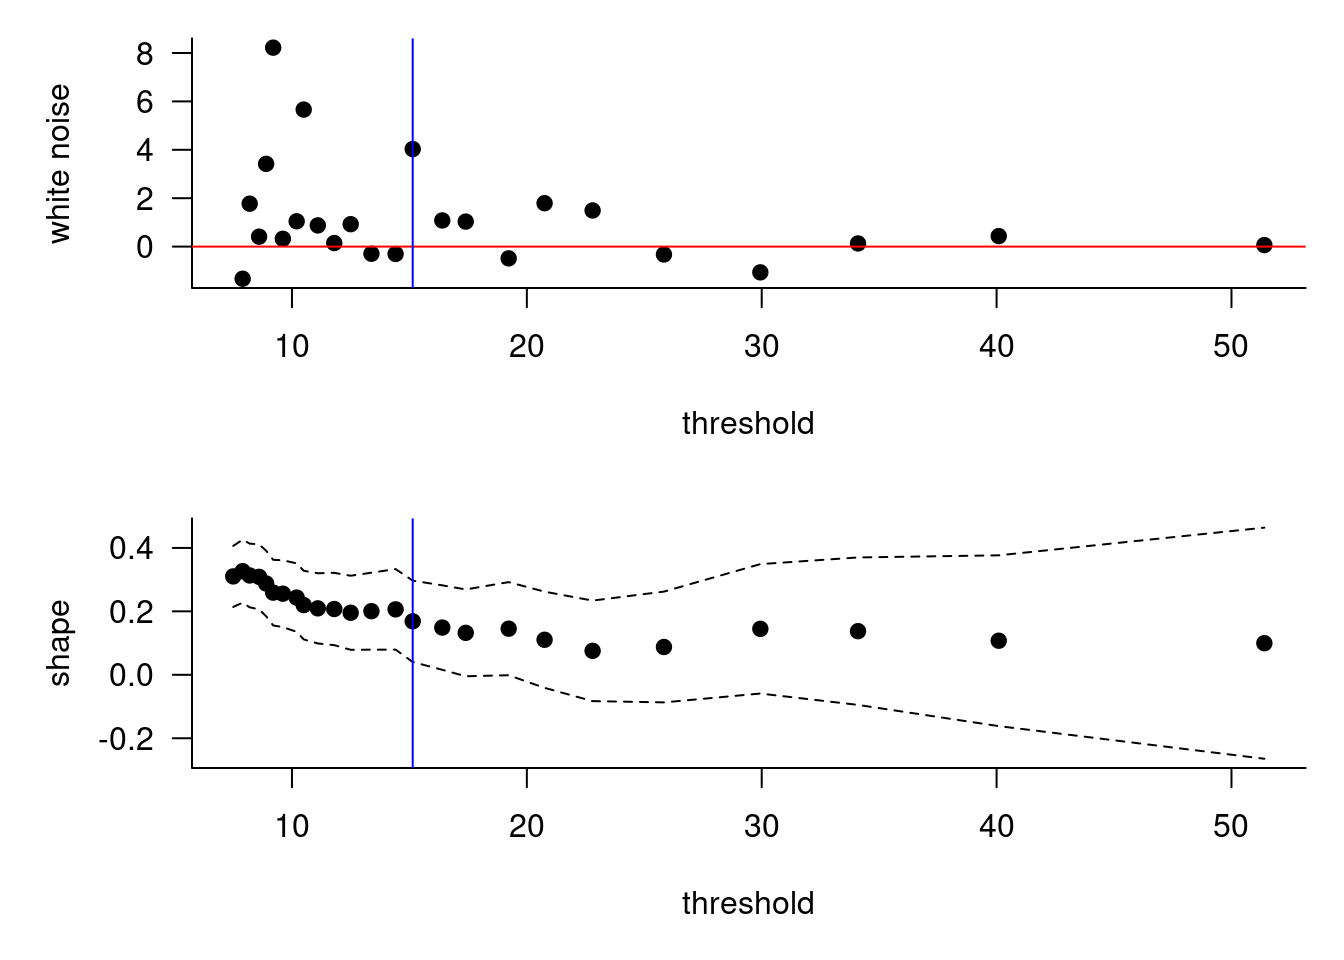
\includegraphics{mevtuto_files/figure-latex/unnamed-chunk-6-1.pdf}

\begin{Shaded}
\begin{Highlighting}[]
\CommentTok{# Profile of median of maxima of 100 years}
\NormalTok{profile <-}\StringTok{ }\KeywordTok{gpd.pll}\NormalTok{(}\DataTypeTok{param =} \StringTok{"Nquant"}\NormalTok{, }\DataTypeTok{dat =}\NormalTok{ nzrain, }\DataTypeTok{threshold =} \DecValTok{15}\NormalTok{, }
        \DataTypeTok{N =} \KeywordTok{length}\NormalTok{(nzrain)}\OperatorTok{/}\NormalTok{(}\DecValTok{1998-1961}\NormalTok{)}\OperatorTok{*}\DecValTok{100}\NormalTok{, }\DataTypeTok{q =} \FloatTok{0.5}\NormalTok{)}
\end{Highlighting}
\end{Shaded}

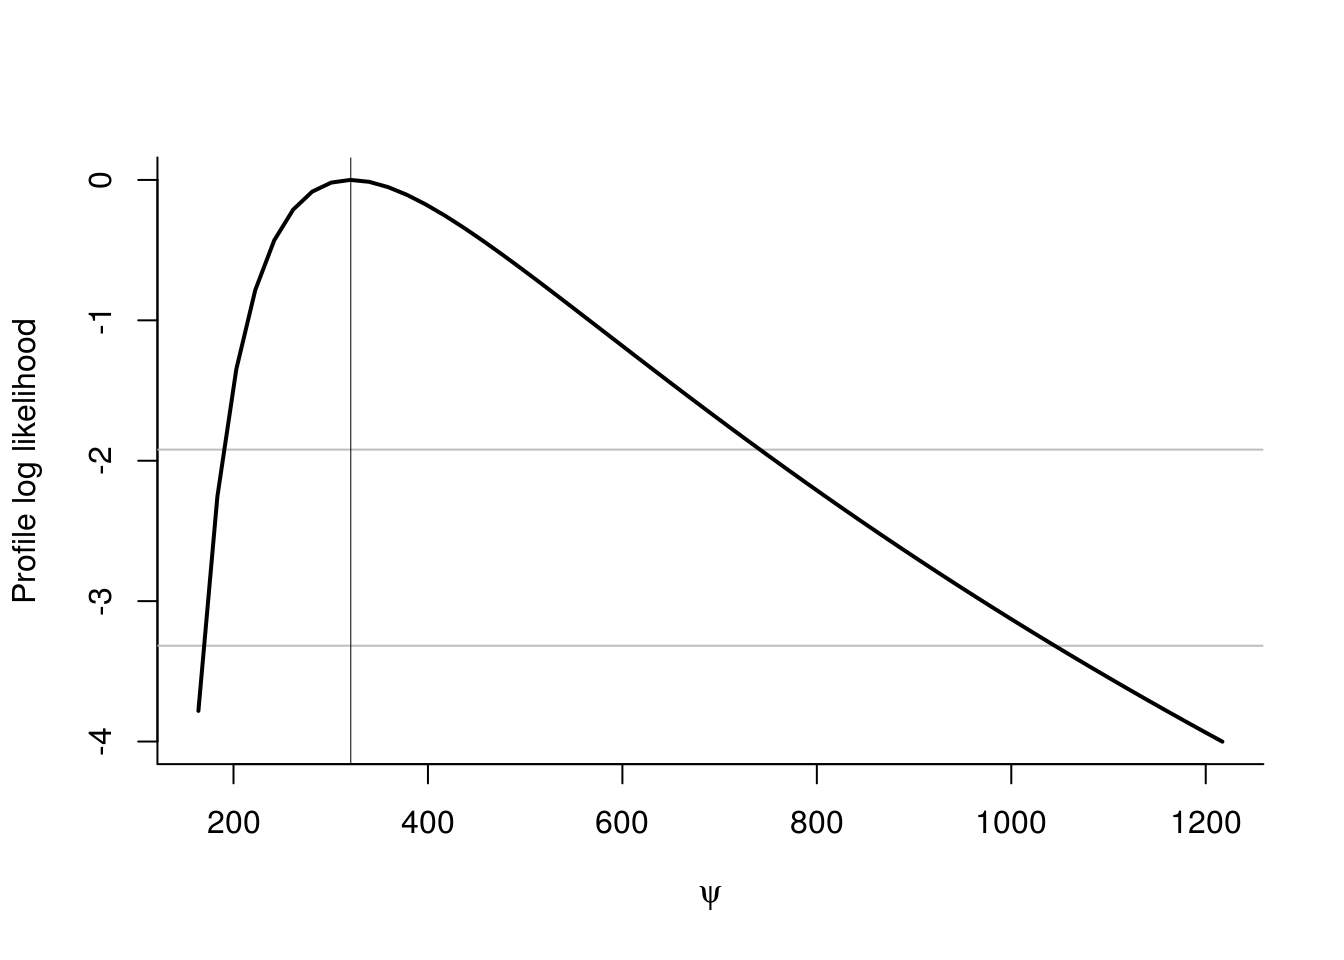
\includegraphics{mevtuto_files/figure-latex/unnamed-chunk-6-2.pdf}

\begin{Shaded}
\begin{Highlighting}[]
\CommentTok{# 95% confidence intervals}
\NormalTok{conf <-}\StringTok{ }\KeywordTok{confint}\NormalTok{(profile, }\DataTypeTok{print =} \OtherTok{TRUE}\NormalTok{)}
\end{Highlighting}
\end{Shaded}

\begin{verbatim}
## Point estimate for the parameter of interest psi:
## Maximum likelihood          : 320.622 
## 
## Confidence intervals, levels : 0.025 0.975 
## Wald intervals               : 118.72 522.524 
## Profile likelihood           : 177.214 741.869
\end{verbatim}

\hypertarget{penultimate-approximation}{%
\chapter{Penultimate approximation}\label{penultimate-approximation}}

The generalized extreme value (GEV) distribution arises as the non-degenerate limiting distribution of maxima. A key property of the generalized extreme value distribution is max-stability, meaning that the distribution of maxima of \(T \in \mathbb{N}\) is the same up to a location-scale transform: if \(F \sim \mathsf{GEV}\), then there exist location and scale constants \(b \in \mathbb{R}\) and \(a>0\) such that \(F^T(ax+b) = F(x)\). The parameters of the new distribution are easily derived: if \(X_i \stackrel{\mathrm{iid}}{\sim}\mathsf{GEV}(\mu,\sigma, \xi)\), then \(\max\{X_1, \ldots, X_T\} \sim \mathsf{GEV}(\mu_T, \sigma_T, \xi)\) with \(\mu_T = \mu - \sigma(1-T^\xi)/\xi\) and \(\sigma_T = \sigma T^\xi\) for \(\xi \neq 0\), or \(\mu_T = \mu +\sigma \log(T)\) and \(\sigma_T = \sigma\) if \(\xi=0\).

In practice, the GEV is fitted to data that are partitioned into \(k\) blocks of (potentially random) sizes \(m_i\). We shall assume that the block sizes are all the same, so that \(m_i=m\) for \(i=1,\ldots, k\) and \(n = km\). The quality of the generalized extreme value approximation increases with the block size \(m\). For fixed block sizes, the estimated shape parameter generally differs from its asymptotic counterpart and this discrepancy usually introduces bias if one extrapolates far beyond the range of the observed data.

Let \(F(x)\) denote a thrice-differentiable distribution function with endpoint \(x^*\) and density \(f(x)\) and define \(s(x)=-F(x)\log\{F(x)\}/f(x)\). The existence of the limit \(\xi_{\infty} = \lim_{n \to \infty} s'\{b_n\}\) is necessary and sufficient for convergence to an extreme value distribution \(G\),
\begin{align*}
 \lim_{n \to \infty} F^n(a_nx+b_n) = \exp\left\{-(1+\xi_\infty x)^{-1/\xi_\infty}\right\}=G(x).
\end{align*}

\citet{Smith:1987} shows that, for any \(x \in \{y:1+\xi_\infty y >0\}\), there exists \(z\) such that
\begin{align*}
   \frac{-\log[F\{v+xs(v)\}]}{-\log\{F(v)\}} = \left\{1+xs'(z)\right\}^{-1/s'(z)}, \qquad v < z < v+xs(v).
\end{align*}
For each \(n \geq 1\), setting \(v=b_n\) and \(a_n=s(b_n)\) yields
\begin{align*}
   F^n(a_nx+b_n)=\exp\left[-\left\{1+s'(z)x\right\}^{-1/s'(z)}\right] + \mathrm{O}(n^{-1})
\end{align*}
for \(z \in [\min(a_nx+b_n, b_n), \max(a_nx+b_n, b_n)]\), depending on the support of \(F\). The ultimate approximation replaces \(s'(z)\) by \(s'(x^*)=\xi_{\infty}\), whereas \citet{Smith:1987} suggests instead suggests taking \(s'(b_n)\), which is closer to \(s'(a_nx+b_n)\) than is \(s'(x^*)\).

The maximum likelihood estimate of the shape should change as the threshold or the block size increases. Consider for simplicity yearly maxima arising from blocking \(m=n_y\) observations per year. We are interested in the distribution of the maximum of \(N\) years and thus the target has roughly shape \(\xi_{Nn_y}\), but our estimates will instead give approximately \(\xi_{n_y}\); an extrapolation error arises from this mismatch between the shape values, which would be constant if the observations were truly max-stable. The curvature of \(s'\) determines how stable the estimates of \(\xi_t\) are when the extrapolation window increases.

We illustrate the previous discussion by looking at block maximum from a log-normal distribution.

\begin{Shaded}
\begin{Highlighting}[]
\KeywordTok{library}\NormalTok{(mev)}
\KeywordTok{set.seed}\NormalTok{(}\DecValTok{123}\NormalTok{)}
\NormalTok{x  <-}\StringTok{ }\KeywordTok{seq}\NormalTok{(}\DecValTok{1}\NormalTok{, }\DecValTok{30}\NormalTok{, }\DataTypeTok{length=}\DecValTok{200}\NormalTok{)}
\NormalTok{fitted <-}\StringTok{ }\KeywordTok{t}\NormalTok{(}\KeywordTok{replicate}\NormalTok{(}\DataTypeTok{n =} \DecValTok{1000}\NormalTok{, }
                      \KeywordTok{fit.gev}\NormalTok{(}\KeywordTok{apply}\NormalTok{(}\KeywordTok{matrix}\NormalTok{(}\KeywordTok{rlnorm}\NormalTok{(}\DecValTok{30}\OperatorTok{*}\DecValTok{100}\NormalTok{), }\DataTypeTok{ncol=} \DecValTok{30}\NormalTok{), }\DecValTok{1}\NormalTok{, max),}
                                        \DataTypeTok{method =} \StringTok{"BFGS"}\NormalTok{)}\OperatorTok{$}\NormalTok{est))}
\NormalTok{penult.bm.lnorm <-}\StringTok{ }\NormalTok{mev}\OperatorTok{::}\KeywordTok{smith.penult}\NormalTok{(}\DataTypeTok{model =} \StringTok{"bm"}\NormalTok{, }\DataTypeTok{m =}\NormalTok{ (m <-}\StringTok{ }\DecValTok{30}\NormalTok{), }\DataTypeTok{family =} \StringTok{"lnorm"}\NormalTok{)}

\KeywordTok{par}\NormalTok{(}\DataTypeTok{mfrow =} \KeywordTok{c}\NormalTok{(}\DecValTok{1}\NormalTok{,}\DecValTok{2}\NormalTok{), }\DataTypeTok{mar =} \KeywordTok{c}\NormalTok{(}\DecValTok{5}\NormalTok{,}\DecValTok{5}\NormalTok{,}\DecValTok{1}\NormalTok{,}\DecValTok{1}\NormalTok{))}
\KeywordTok{hist}\NormalTok{(fitted[,}\DecValTok{3}\NormalTok{], }\DataTypeTok{probability =} \OtherTok{TRUE}\NormalTok{, }\DataTypeTok{breaks =} \DecValTok{20}\NormalTok{, }
     \DataTypeTok{xlab =} \StringTok{"Estimated shape"}\NormalTok{, }\DataTypeTok{main =} \StringTok{""}\NormalTok{)}
\KeywordTok{segments}\NormalTok{(}\DataTypeTok{y0 =} \FloatTok{-0.5}\NormalTok{, }\DataTypeTok{y1 =} \DecValTok{0}\NormalTok{, }\DataTypeTok{x0 =}\NormalTok{ penult.bm.lnorm}\OperatorTok{$}\NormalTok{shape, }\DataTypeTok{col =} \StringTok{"red"}\NormalTok{, }\DataTypeTok{lwd =} \DecValTok{2}\NormalTok{)}
\KeywordTok{segments}\NormalTok{(}\DataTypeTok{y0 =} \FloatTok{-0.5}\NormalTok{, }\DataTypeTok{y1 =} \DecValTok{0}\NormalTok{, }\DataTypeTok{x0 =} \DecValTok{0}\NormalTok{, }\DataTypeTok{col =} \StringTok{"black"}\NormalTok{, }\DataTypeTok{lwd =} \DecValTok{2}\NormalTok{)}

\NormalTok{p30 <-}\StringTok{ }\NormalTok{penult.bm.lnorm}
\NormalTok{x =}\StringTok{ }\KeywordTok{seq}\NormalTok{(}\DecValTok{0}\NormalTok{,}\DecValTok{100}\NormalTok{, }\DataTypeTok{length =} \DecValTok{400}\NormalTok{)}
\NormalTok{N <-}\StringTok{ }\DecValTok{1000}\NormalTok{; N30 =}\StringTok{ }\NormalTok{N}\OperatorTok{/}\DecValTok{30}
\KeywordTok{plot}\NormalTok{(x, N}\OperatorTok{*}\KeywordTok{exp}\NormalTok{((N}\DecValTok{-1}\NormalTok{)}\OperatorTok{*}\KeywordTok{plnorm}\NormalTok{(x, }\DataTypeTok{log.p=}\OtherTok{TRUE}\NormalTok{))}\OperatorTok{*}
\StringTok{       }\KeywordTok{dlnorm}\NormalTok{(x), }
     \DataTypeTok{type=}\StringTok{"l"}\NormalTok{, }\DataTypeTok{bty =} \StringTok{"l"}\NormalTok{, }\DataTypeTok{ylim =} \KeywordTok{c}\NormalTok{(}\DecValTok{0}\NormalTok{,}\FloatTok{0.1}\NormalTok{),}
     \DataTypeTok{xlab=}\StringTok{"x"}\NormalTok{, }\DataTypeTok{ylab=}\StringTok{"Density"}\NormalTok{)}
\CommentTok{# Get parameters of maximum of N GEV}
\NormalTok{maxstabp <-}\StringTok{ }\ControlFlowTok{function}\NormalTok{(loc, scale, shape, N)\{}
   \ControlFlowTok{if}\NormalTok{(}\OperatorTok{!}\KeywordTok{isTRUE}\NormalTok{(}\KeywordTok{all.equal}\NormalTok{(shape, }\DecValTok{0}\NormalTok{, }\DataTypeTok{check.attributes =} \OtherTok{FALSE}\NormalTok{)))\{}
\NormalTok{      mut <-}\StringTok{ }\NormalTok{loc }\OperatorTok{-}\StringTok{ }\NormalTok{scale}\OperatorTok{*}\NormalTok{(}\DecValTok{1}\OperatorTok{-}\NormalTok{N}\OperatorTok{^}\NormalTok{shape)}\OperatorTok{/}\NormalTok{shape}
\NormalTok{      sigmat =}\StringTok{ }\NormalTok{scale}\OperatorTok{*}\NormalTok{N}\OperatorTok{^}\NormalTok{shape}
      \KeywordTok{return}\NormalTok{(}\KeywordTok{c}\NormalTok{(}\DataTypeTok{loc =}\NormalTok{ mut, }\DataTypeTok{scale =}\NormalTok{ sigmat, }\DataTypeTok{shape =}\NormalTok{ shape))}
\NormalTok{   \} }\ControlFlowTok{else}\NormalTok{\{}
\NormalTok{      mut <-}\StringTok{ }\NormalTok{loc }\OperatorTok{+}\StringTok{ }\NormalTok{scale}\OperatorTok{*}\KeywordTok{log}\NormalTok{(N)}
       \KeywordTok{return}\NormalTok{(}\KeywordTok{c}\NormalTok{(}\DataTypeTok{loc =}\NormalTok{ mut, }\DataTypeTok{scale =}\NormalTok{ scale, }\DataTypeTok{shape =}\NormalTok{ shape))}
\NormalTok{   \}}
\NormalTok{ \}}
\NormalTok{p30e <-}\StringTok{ }\KeywordTok{maxstabp}\NormalTok{(}\DataTypeTok{loc =}\NormalTok{ p30}\OperatorTok{$}\NormalTok{loc, }\DataTypeTok{scale =}\NormalTok{ p30}\OperatorTok{$}\NormalTok{scale, }\DataTypeTok{shape =}\NormalTok{ p30}\OperatorTok{$}\NormalTok{shape, }\DataTypeTok{N =}\NormalTok{ N30)}
\KeywordTok{lines}\NormalTok{(x, evd}\OperatorTok{::}\KeywordTok{dgev}\NormalTok{(x, }\DataTypeTok{loc =}\NormalTok{ p30e[}\StringTok{'loc'}\NormalTok{],}
              \DataTypeTok{scale =}\NormalTok{ p30e[}\StringTok{'scale'}\NormalTok{], }
              \DataTypeTok{shape =}\NormalTok{ p30e[}\StringTok{'shape'}\NormalTok{]), }
      \DataTypeTok{col =} \StringTok{"red"}\NormalTok{, }\DataTypeTok{lwd =} \DecValTok{2}\NormalTok{, }\DataTypeTok{lty =} \DecValTok{2}\NormalTok{)}
\NormalTok{p30l <-}\StringTok{ }\KeywordTok{maxstabp}\NormalTok{(}\DataTypeTok{loc =}\NormalTok{ p30}\OperatorTok{$}\NormalTok{loc, }\DataTypeTok{scale =}\NormalTok{ p30}\OperatorTok{$}\NormalTok{scale, }\DataTypeTok{shape =} \DecValTok{0}\NormalTok{, }\DataTypeTok{N =}\NormalTok{ N30)}
\KeywordTok{lines}\NormalTok{(x, evd}\OperatorTok{::}\KeywordTok{dgev}\NormalTok{(x, }
                   \DataTypeTok{loc =}\NormalTok{ p30e[}\StringTok{'loc'}\NormalTok{], }
                   \DataTypeTok{scale =}\NormalTok{ p30l[}\StringTok{'scale'}\NormalTok{], }
                   \DataTypeTok{shape =} \DecValTok{0}\NormalTok{), }\DataTypeTok{col =} \DecValTok{1}\NormalTok{, }\DataTypeTok{lty=}\DecValTok{3}\NormalTok{, }\DataTypeTok{lwd=}\DecValTok{1}\NormalTok{)}
\KeywordTok{legend}\NormalTok{(}\DataTypeTok{x =} \StringTok{"topright"}\NormalTok{, }
       \DataTypeTok{legend =} \KeywordTok{c}\NormalTok{(}\StringTok{"exact"}\NormalTok{,}\StringTok{"ultimate"}\NormalTok{, }\StringTok{"penultimate"}\NormalTok{), }
       \DataTypeTok{col =} \KeywordTok{c}\NormalTok{(}\DecValTok{1}\NormalTok{,}\DecValTok{1}\NormalTok{,}\DecValTok{2}\NormalTok{), }
       \DataTypeTok{lwd =} \KeywordTok{c}\NormalTok{(}\DecValTok{2}\NormalTok{,}\DecValTok{2}\NormalTok{,}\DecValTok{1}\NormalTok{), }\DataTypeTok{bty =} \StringTok{"n"}\NormalTok{, }
       \DataTypeTok{lty =} \KeywordTok{c}\NormalTok{(}\DecValTok{1}\NormalTok{,}\DecValTok{3}\NormalTok{,}\DecValTok{2}\NormalTok{))}
\end{Highlighting}
\end{Shaded}

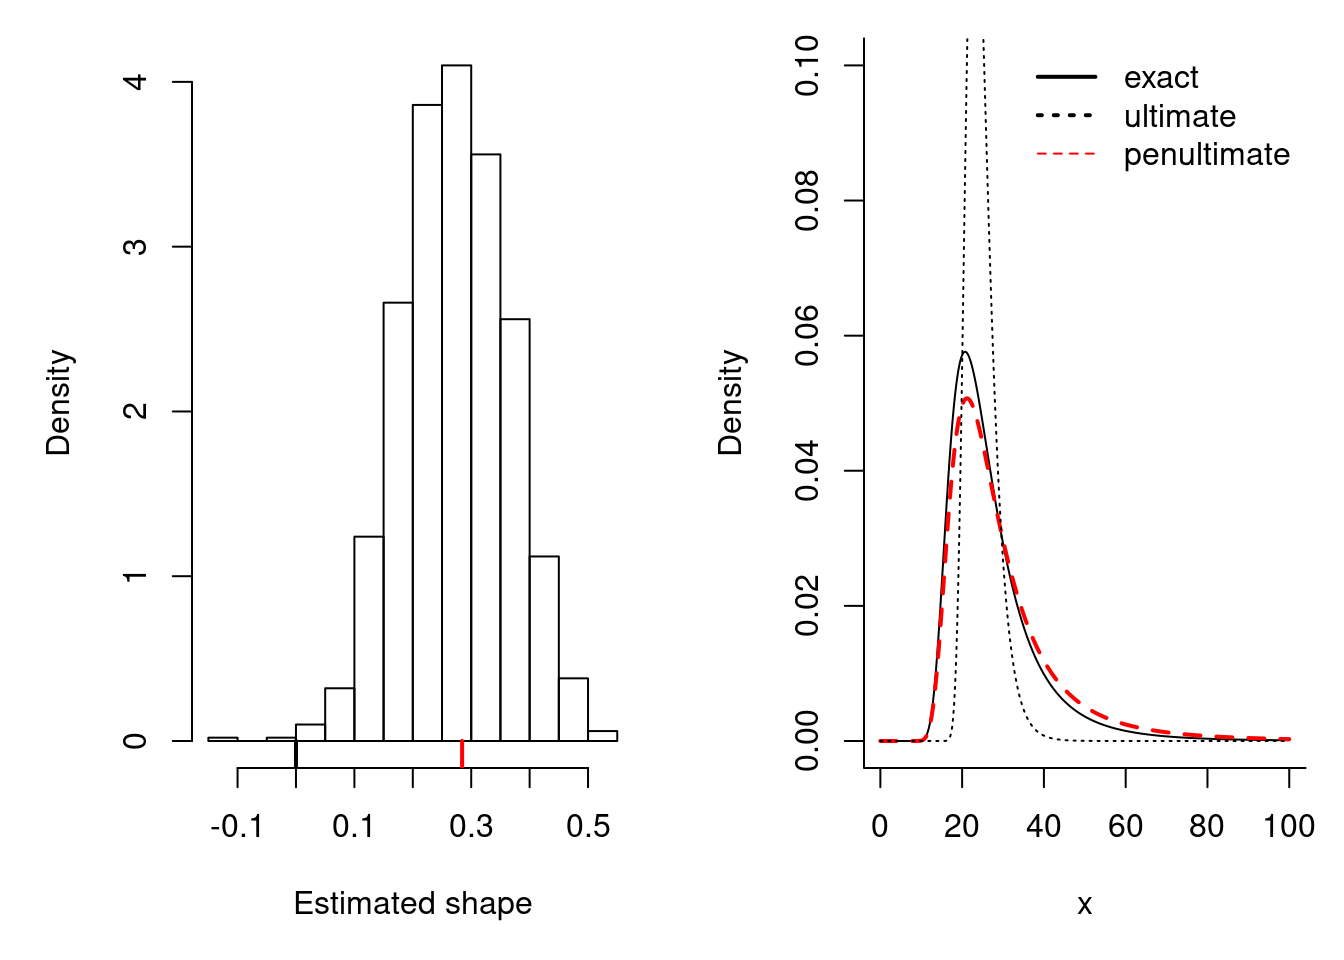
\includegraphics{mevtuto_files/figure-latex/unnamed-chunk-7-1.pdf}

The left panel illustrates how maximum likelihood estimates of the parameters for repeated samples from a log-normal distribution are closer to the penultimate approximation than to the limiting tail index \(\xi_{\infty}=0\). Using max-stability, we could get an estimate of the distribution of the maximum of \(Nn_y\) observations. In this case, the penultimate shape for \(m=1000\) is approximately \(\xi_{1000}=0.215\), compared to \(\xi_{30} \approx 0.284\), which is far from the limiting value \(\xi_{\infty}=0\). The extrapolated density estimate is based on \(F_1^{1000/30}\), the generalized extreme value density associated to the distribution function of the penultimate approximation \(F_1^{1000/30}\), with \(F_1 \sim\mathsf{GEV}(a_{30}, b_{30}, \xi_{30})\). The penultimate approximation \(F_2\) is more accurate than the ultimate approximation \(\mathsf{GEV}(a_{30}, b_{30}, \xi_\infty)\), which is too short tailed.

The function \texttt{smith.penult} computes the penultimate approximation for parameter models in \textbf{R} for the distribution assuming a model \texttt{family} with arguments \texttt{dfamily}, \texttt{qfamily} and \texttt{pfamily} exist. It returns the penultimate parameters for a given block size or quantile in case of threshold models. These functions are particularly useful for simulation studies in which one wants to obtain an approximation for \(F^N\) for large \(N\), to get an approximation to the asymptotic distribution of a test statistic for finite \(N\); the \(\mathsf{GEV}\) penultimate approximation is more numerically stable for certain models and its moments and cumulants are easily derived.

The following plot illustrates the penultimate shape parameter for the normal distribution based on threshold exceedances. In finite samples, the upper tail is bounded, but the quality of the approximation by the Gumbel distribution increases as \(u \to \infty\), albeit very slowly.

\begin{Shaded}
\begin{Highlighting}[]
\NormalTok{penult <-}\StringTok{ }\KeywordTok{smith.penult}\NormalTok{(}\DataTypeTok{family =} \StringTok{"norm"}\NormalTok{, }\DataTypeTok{method =} \StringTok{"pot"}\NormalTok{, }
                       \DataTypeTok{u =} \KeywordTok{qnorm}\NormalTok{(u <-}\StringTok{ }\KeywordTok{seq}\NormalTok{(}\FloatTok{0.8}\NormalTok{, }\FloatTok{0.9999}\NormalTok{, }\DataTypeTok{by =} \FloatTok{0.0001}\NormalTok{))) }
\KeywordTok{plot}\NormalTok{(u, penult}\OperatorTok{$}\NormalTok{shape, }\DataTypeTok{bty =} \StringTok{"l"}\NormalTok{, }\DataTypeTok{type=}\StringTok{'l'}\NormalTok{, }\DataTypeTok{xlab=}\StringTok{'Quantile'}\NormalTok{, }\DataTypeTok{ylab=}\StringTok{'Penultimate shape'}\NormalTok{)}
\end{Highlighting}
\end{Shaded}

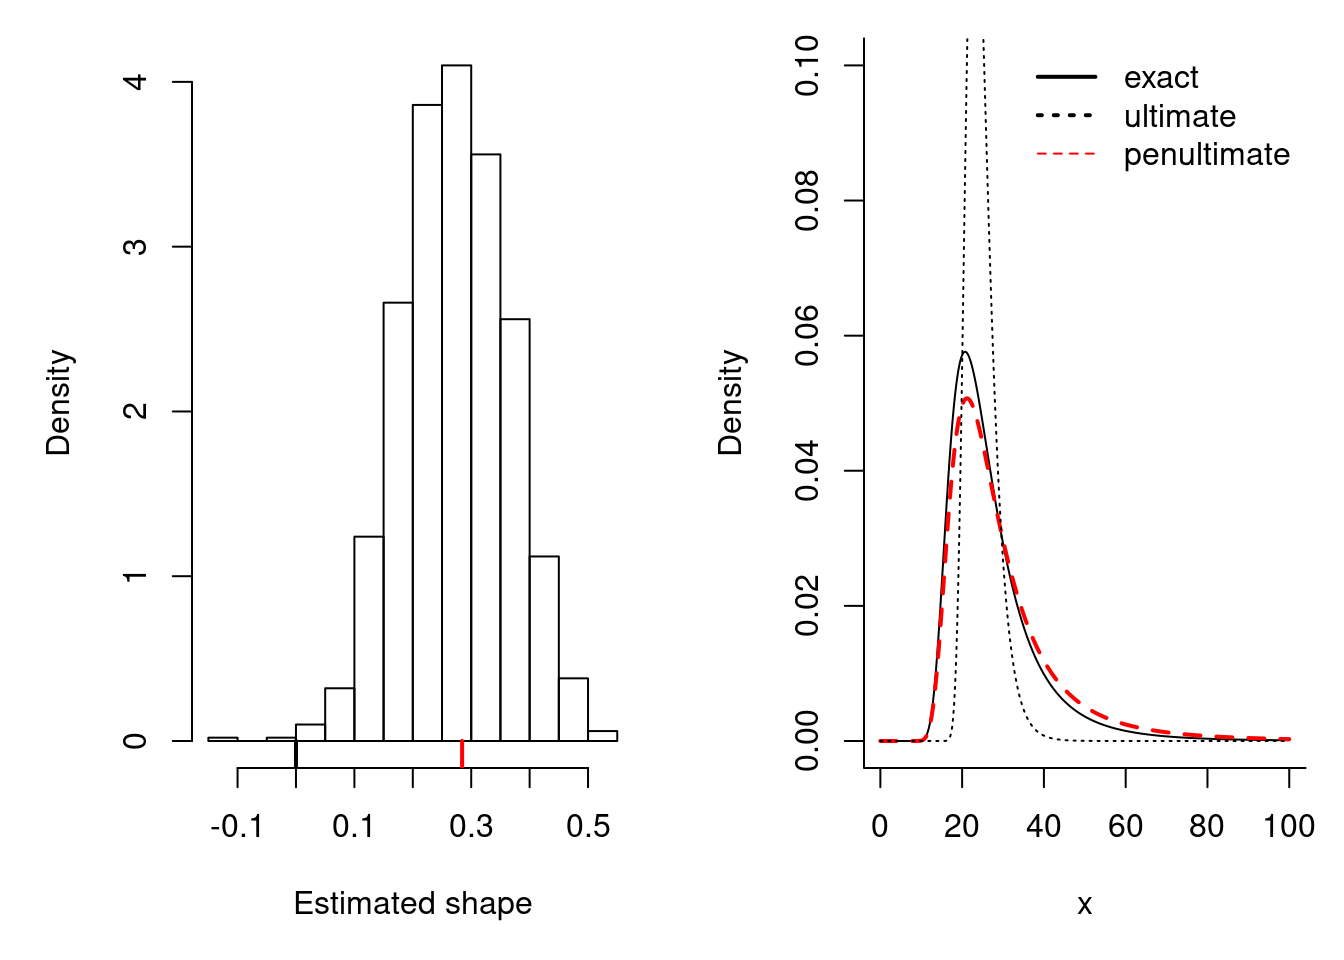
\includegraphics{mevtuto_files/figure-latex/unnamed-chunk-8-1.pdf}

\hypertarget{threshold-selection}{%
\chapter{Threshold selection}\label{threshold-selection}}

The generalized Pareto (GP) distribution with scale \(\sigma \in \mathbb{R}_{+}\) and shape \(\xi \in \mathbb{R}\) is
\begin{align*}
  G(x)  = \begin{cases}
1-\left\{1+\xi \left(\frac{x}{\sigma}\right)\right\}_{+}^{-1/\xi}, &  \xi \neq 0,
\\ 1-\exp \left(-{x}{\sigma}\right),&  \xi = 0.
\end{cases}
 \end{align*}
The range of the generalized Pareto distribution is \([0, -\sigma/\xi)\) if \(\xi < 0\) and \(\mathbb{R}_{+}\) otherwise.

Why is the generalized Pareto distribution so central to peaks-over-threshold analysis? The conditional distribution of exceedances over a threshold \(u < x^*\) converges to a generalized Pareto distribution as \(u\) converges to the endpoint of the distribution,
\begin{align*}
\lim_{u \to x^*} \frac{1-F(xa_u+u)}{1-F(u)} = 1-H(x),
\end{align*}
where \(H(x)\) is the distribution function of \(\mathsf{GP}(1, \xi)\).

If \(X \sim \mathsf{GP}(\sigma, \xi)\), straightforward calculations show that \(X-u \mid X>u \sim \mathsf{GP}(\sigma + \xi u, \xi)\) for any \(u \in \mathbb{R}\) such that \(\sigma+\xi u>0\), meaning that conditional exceedances above a threshold \(u\) also follow a generalized Pareto distribution. This property is termed threshold-stability.

The limiting distribution of threshold exceedances is generalized Pareto as \(u \to x^*\) but, in practice, we must choose a finite threshold in order to have enough exceedances to draw inference. Since the scaling constant \(a_u\) is unknown, we have \(X \mid X > u \stackrel{\cdot}{\sim} \mathsf{GP}(\sigma_u, \xi)\). The term \(1-F(u)\) in the denominator is the fraction of points exceeding the threshold, which has a binomial distribution.

Threshold selection is subtle and it is common to select a high percentile of the data, say the
95\% value, as the threshold, even if this is asymptotically incorrect, as in this case \(k/n \nrightarrow 0\) as \(n \to \infty\). Most approaches for threshold selection rely on properties of the
generalized Pareto distribution (moments, threshold-stability) to determine a region within which the asymptotic distribution fits the data well and the parameter estimates are stable.

Below, we focus on recent graphical selection tools for likelihood based inference; mixture models are reviewed in \citet{Scarrott:2012} and are available in the package \texttt{evmix}.

\hypertarget{robust-selection}{%
\section{Robust selection}\label{robust-selection}}

The extreme value distributions have unbounded influence functions and outliers can strongly affect the estimate of the shape. \citet{Dupuis:1999} proposes an optimal \(B\)-robust estimator of the generalized Pareto parameters. Points that are outlying or for which the fit is poor are downweighted; if the weights for the largest observations are very low, this suggests that the threshold is too low. While there is no guarantee that observations that were simulated from a generalized Pareto distributed would not be downweighted, systematic downweighting of the largest exceedances may be indicative of poor fit.

\hypertarget{threshold-stability-plots}{%
\section{Threshold stability plots}\label{threshold-stability-plots}}

Consider a sequence of ordered candidate thresholds \(u_1 < \cdots < u_k\); one of the most widely used tools for threshold selection is the threshold-stability plots of \citet{Davison:1990}. These show the point estimates of the shape \(\xi\) and the modified scale \(\sigma_{u_i}-\xi u_i\), which should be constant for any threshold \(u_{j} >u_i\) assuming that the generalized Pareto above \(u_i\) holds exactly. In addition to the point estimates, the asymptotic pointwise 95\% Wald confidence intervals are displayed; the standard errors are obtained from the observed information matrix. While these are displayed by many packages, notably \texttt{extRemes}, \texttt{ismev} and \texttt{evd} , \texttt{mev} allows you to use profile likelihood based confidence intervals, which typically offer better coverage and capture some of the asymmetry of the distribution. The \texttt{mev} package functions for producing threshold stability plots are \texttt{tstab.gpd} and \texttt{tstab.pp} for respectively the generalized Pareto and Poisson process likelihoods.

Parameter stability plots can be difficult to interpret because the confidence intervals are pointwise rather than simultaneous (each fit likewise uses an overlapping portion of the data). The plots also ignore changes in the estimated parameters due to the penultimate approximation.

\hypertarget{wadsworths-diagnostics-white-noise-process-and-simultaneous-threshold-stability-plots}{%
\section{Wadsworth's diagnostics: white noise process and simultaneous threshold stability plots}\label{wadsworths-diagnostics-white-noise-process-and-simultaneous-threshold-stability-plots}}

The problem with the threshold stability plots lies in the point-wise nature of the estimate. Assuming a superposition of \(k\) Poisson processes, \citet{Wadsworth:2016} derives the limiting distribution of the maximum likelihood estimators from the Poisson process for overlapping windows as the number of windows \(k \to \infty\) and \(n_k \to \infty\). The joint asymptotic Gaussian distribution allows \citet{Wadsworth:2016} to propose two additional diagnostics: a white noise sequence of differences in estimates of the shape, standardized to have unit variance. The variables \(\xi^*_i=(\hat{\xi}_{u_{i+1}}-\hat{\xi}_{u_i})/\{(I^{-1}_{u_{i+1}}-I^{-1}_{u_{i}})_{\xi,\xi}^{1/2}\}\), where \(I_{u_{i}}\) is the Fisher information of the Poisson process likelihood for exceedances above \(u_i\), should form a white-noise sequence of independent variables centered around the origin; systematic deviations are indicative of inadequacy. To formally test the hypothesis, a likelihood ratio test can be used assuming a simple alternative, namely a single change point at threshold \(u_j\). The null hypothesis is \(\mathrm{H}_0: \xi_i^* \stackrel{\mathrm{iid}}{\sim}\textsf{No}(0,1)\) for \(i=1, \ldots, k-1\) against the alternative \(\mathrm{H}_a: \xi^*_i \sim \textsf{No}(\beta, \sigma) (i=1, \ldots, j-1)\) and \(\xi^*_i \sim \textsf{No}(0,1)\) for \(j, \ldots, k-1\). This alternative is motivated by results on model misspecification \citep{White:1982}, which suggest that the asymptotic distribution may still be Gaussian, but with a different mean and variance. This can be used to automate threshold selection, by picking the smallest threshold for which the \(P\)-value is above the level \(\alpha\). The function \texttt{W.diag} returns diagnostics plots (for the likelihood ratio statistic path, the white noise process and threshold stability along with asymptotic simultaneous confidence intervals) for non-homogeneous Poisson process model and for the bivariate exponential and the over a sequence of thresholds, specified using \texttt{q1}, \texttt{q2} and \texttt{k}. The argument \texttt{M} is a tuning parameter that can be chosen in a way such that the parameters of the non-homogeneous Poisson process likelihood coincide with those of the generalized extreme value distribution for blocks of size \(m\); see \citet{Coles:2001} to this effect.

A main criticism of the proposals of \citet{Wadsworth:2016} is their lack of robustness. For the asymptotic result to be approximately valid, the number of thresholds must be large, which implicitly requires large samples for each superposed point process. Moreover, the estimated difference in Fisher information matrices often fails to be positive definite in practice. The procedure is highly sensitive to the choice of \(k\). Changing the set of thresholds \(\boldsymbol{u}\) under consideration leads to potentially completely different parameter estimates being chosen by the automated procedure.

\hypertarget{changepoint-tests-based-on-penultimate-approximation}{%
\section{Changepoint tests based on penultimate approximation}\label{changepoint-tests-based-on-penultimate-approximation}}

Let \(F(x)\) denote a thrice-differentiable distribution function with endpoint \(x^*\) and density \(f(x)\). Define the reciprocal hazard function \(r(x) = \{1-F(x)\}/f(x)\).
The existence of the limit \(\xi_{\infty} = \lim_{n \to \infty} s'\{b_n\}\) is necessary and sufficient for convergence to an extreme value distribution and \citet{Smith:1987} shows that there exists \(y\) such that
\begin{align*}
 \frac{1-F\{u+xr(u)\}}{1-F(u)} = \left\{1+xr'(y)\right\}_{+}^{-1/r'(y)}, \qquad u < y < u+xr(u),
\end{align*}
unless \(r'(x)\) is constant. The penultimate shape parameter for the generalized Pareto distribution is \(r'(u)\), but the true shape parameter lies between \(r'(u)\) and \(\xi_{\infty}\).

When we fit the limiting parametric models to finite samples, maximum likelihood estimates of the shape parameter will be closer to their penultimate counterparts than to the limiting value and we can expect them to vary as we increase the threshold.

\citet{Northrop:2014} adapt the idea of \citet{Wadsworth:2012} and fit a generalized Pareto model with piecewise constant shape to \(k\) different thresholds; continuity constraints at the thresholds impose \(k-1\) restrictions on scale parameters, so the model only has \(k+1\) parameters. A score test can be used to test the hypothesis of equal shape and it only requires evaluation of the model under the null hypothesis that a generalized Pareto distribution is valid above all thresholds. A diagnostic plot is obtained by plotting \(P\)-values against threshold. One can then choose to take, e.g., (a) the lowest threshold at which the \(P\)-value is non-significant, or (b) the lowest threshold at which the \(P\)-values for all higher thresholds are non-significant: under the null hypothesis, there is an \(\alpha\%\) probability of rejection at any given threshold. The function \texttt{NC.diag} computes the \(P\)-value of the score test as a function of the threshold.

\hypertarget{extended-generalized-pareto}{%
\section{Extended generalized Pareto}\label{extended-generalized-pareto}}

\citet{Papastathopoulos:2013} propose three extended generalized Pareto distributions: for example, the third extended generalized Pareto model has distribution function \(\{1-(1+\xi x/\sigma)^{-1/\xi}_{+}\}^{\kappa}\) for \(x >0\) and \(\kappa > 0\). Each family reduces to the generalized Pareto when the additional parameter \(\kappa=1\) and share the same tail index \(\xi\), the extended generalized Pareto provide more flexibility for modelling departures from the limiting form. Standard parameter stability plots can be used to find a region in which \(\kappa \approx 1\) and the shape parameter stabilizes. The additional parameter gives flexibility for modelling departures from the limiting distribution and the hope is one can fit to exceedances over lower threshold and increase the number of points to which the distribution is fitted. The stability plots, obtained through \texttt{tstab.egp}, suffer from the same caveats as classical diagnostics.

\hypertarget{simulation}{%
\chapter{Simulation}\label{simulation}}

The original goal of the \texttt{mev} package was to implement the algorithm of \citet{Dombry:2016} in order to perform exact simulation from max-stable vectors. Since then, other algorithms for simulating from standard \(R\)-Pareto processes and generalized \(R\)-Pareto processes have been implemented. These are based on accept-reject method or composition sampling.

Let's start by simulating from a simple max-stable random vector from the negative logistic model. The margins are unit Frechet, and we can verify this by pooling the observations and fitting a generalized extreme value distribution to the sample.

\begin{Shaded}
\begin{Highlighting}[]
\KeywordTok{library}\NormalTok{(mev)}
\KeywordTok{set.seed}\NormalTok{(}\DecValTok{1234}\NormalTok{)}
\NormalTok{samp <-}\StringTok{ }\KeywordTok{rmev}\NormalTok{(}\DataTypeTok{n =} \DecValTok{1000}\NormalTok{, }\DataTypeTok{d =} \DecValTok{5}\NormalTok{, }\DataTypeTok{param =} \FloatTok{0.1}\NormalTok{, }\DataTypeTok{model =} \StringTok{"neglog"}\NormalTok{) }
\KeywordTok{fit.gev}\NormalTok{(}\KeywordTok{c}\NormalTok{(samp), }\DataTypeTok{show =} \OtherTok{FALSE}\NormalTok{)}\OperatorTok{$}\NormalTok{estimate}
\end{Highlighting}
\end{Shaded}

\begin{verbatim}
##      loc    scale    shape 
## 0.994592 1.001284 1.035500
\end{verbatim}

We simulate a spatial generalized \(R\)-Pareto process.

\begin{Shaded}
\begin{Highlighting}[]
\NormalTok{ lon <-}\StringTok{ }\KeywordTok{seq}\NormalTok{(}\DecValTok{650}\NormalTok{, }\DecValTok{720}\NormalTok{, }\DataTypeTok{length =} \DecValTok{50}\NormalTok{)}
\NormalTok{ lat <-}\StringTok{ }\KeywordTok{seq}\NormalTok{(}\DecValTok{215}\NormalTok{, }\DecValTok{290}\NormalTok{, }\DataTypeTok{length =} \DecValTok{50}\NormalTok{)}
 \CommentTok{# Create a grid}
\NormalTok{ grid <-}\StringTok{ }\KeywordTok{expand.grid}\NormalTok{(lon,lat)}
\NormalTok{ coord <-}\StringTok{ }\KeywordTok{as.matrix}\NormalTok{(grid)}
\NormalTok{ dianiso <-}\StringTok{ }\KeywordTok{distg}\NormalTok{(coord, }\FloatTok{1.5}\NormalTok{, }\FloatTok{0.5}\NormalTok{)}
\NormalTok{ sgrid <-}\StringTok{ }\KeywordTok{scale}\NormalTok{(grid, }\DataTypeTok{scale =} \OtherTok{FALSE}\NormalTok{)}
 \CommentTok{# Specify marginal parameters `loc` and `scale` over grid}
\NormalTok{ eta <-}\StringTok{ }\DecValTok{26} \OperatorTok{+}\StringTok{ }\FloatTok{0.05}\OperatorTok{*}\NormalTok{sgrid[,}\DecValTok{1}\NormalTok{] }\OperatorTok{-}\StringTok{ }\FloatTok{0.16}\OperatorTok{*}\NormalTok{sgrid[,}\DecValTok{2}\NormalTok{]}
\NormalTok{ tau <-}\StringTok{ }\DecValTok{9} \OperatorTok{+}\StringTok{ }\FloatTok{0.05}\OperatorTok{*}\NormalTok{sgrid[,}\DecValTok{1}\NormalTok{] }\OperatorTok{-}\StringTok{ }\FloatTok{0.04}\OperatorTok{*}\NormalTok{sgrid[,}\DecValTok{2}\NormalTok{]}
 \CommentTok{# Parameter matrix of Huesler--Reiss}
 \CommentTok{# associated to power variogram}
\NormalTok{ Lambda <-}\StringTok{ }\NormalTok{((dianiso}\OperatorTok{/}\DecValTok{30}\NormalTok{)}\OperatorTok{^}\FloatTok{0.7}\NormalTok{)}\OperatorTok{/}\DecValTok{4}
 \CommentTok{# Simulate generalized max-Pareto field above u=50}
 \KeywordTok{set.seed}\NormalTok{(}\DecValTok{345}\NormalTok{)}
\NormalTok{ simu1 <-}\StringTok{ }\KeywordTok{rgparp}\NormalTok{(}\DataTypeTok{n =} \DecValTok{1}\NormalTok{, }\DataTypeTok{thresh =} \DecValTok{50}\NormalTok{, }\DataTypeTok{shape =} \FloatTok{0.1}\NormalTok{, }\DataTypeTok{riskf =} \StringTok{"max"}\NormalTok{,}
                 \DataTypeTok{scale =}\NormalTok{ tau, }\DataTypeTok{loc =}\NormalTok{ eta, }\DataTypeTok{sigma =}\NormalTok{ Lambda, }\DataTypeTok{model =} \StringTok{"hr"}\NormalTok{)}
\CommentTok{# The same, but conditional on an exceedance at a site    }
\NormalTok{simu2 <-}\StringTok{ }\KeywordTok{rgparp}\NormalTok{(}\DataTypeTok{n =} \DecValTok{1}\NormalTok{, }\DataTypeTok{thresh =} \DecValTok{50}\NormalTok{, }\DataTypeTok{shape =} \FloatTok{0.1}\NormalTok{, }\DataTypeTok{riskf =} \StringTok{"site"}\NormalTok{, }
                \DataTypeTok{siteindex =} \DecValTok{1225}\NormalTok{, }\DataTypeTok{scale =}\NormalTok{ tau, }\DataTypeTok{loc =}\NormalTok{ eta,}
                \DataTypeTok{sigma =}\NormalTok{ Lambda, }\DataTypeTok{model =} \StringTok{"hr"}\NormalTok{)}
\CommentTok{#Plot the generalized max-Pareto field}
\KeywordTok{par}\NormalTok{(}\DataTypeTok{mfrow =} \KeywordTok{c}\NormalTok{(}\DecValTok{1}\NormalTok{,}\DecValTok{2}\NormalTok{))}
\NormalTok{fields}\OperatorTok{::}\KeywordTok{quilt.plot}\NormalTok{(grid[,}\DecValTok{1}\NormalTok{], grid[,}\DecValTok{2}\NormalTok{], simu1, }\DataTypeTok{nx =} \DecValTok{50}\NormalTok{, }\DataTypeTok{ny =} \DecValTok{50}\NormalTok{)}
\NormalTok{SpatialExtremes}\OperatorTok{::}\KeywordTok{swiss}\NormalTok{(}\DataTypeTok{add =} \OtherTok{TRUE}\NormalTok{)}
\NormalTok{fields}\OperatorTok{::}\KeywordTok{quilt.plot}\NormalTok{(grid[,}\DecValTok{1}\NormalTok{], grid[,}\DecValTok{2}\NormalTok{], simu2, }\DataTypeTok{nx =} \DecValTok{50}\NormalTok{, }\DataTypeTok{ny =} \DecValTok{50}\NormalTok{)}
\NormalTok{SpatialExtremes}\OperatorTok{::}\KeywordTok{swiss}\NormalTok{(}\DataTypeTok{add =} \OtherTok{TRUE}\NormalTok{)}
\end{Highlighting}
\end{Shaded}

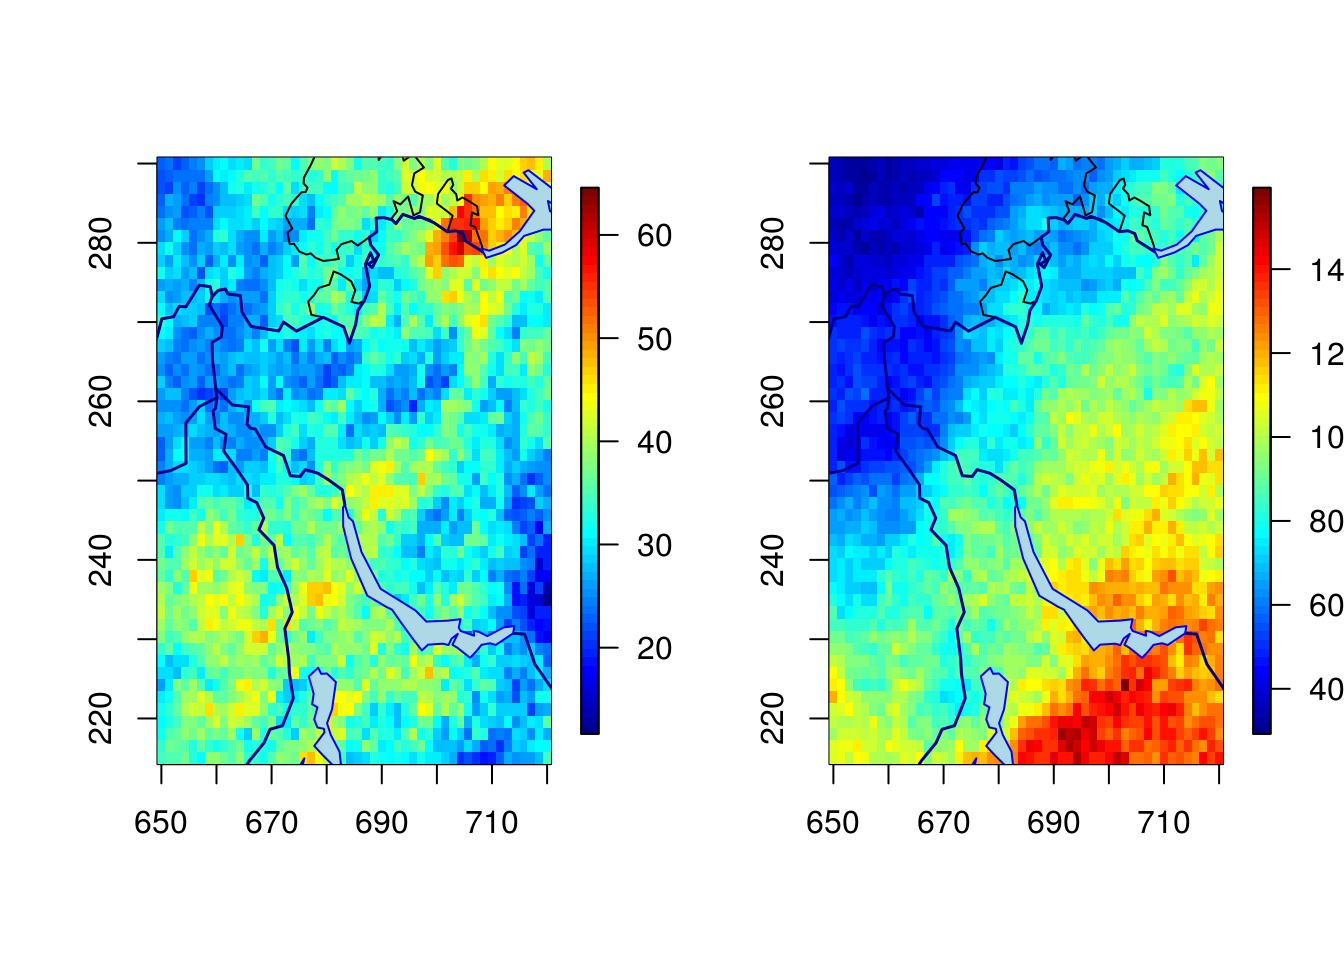
\includegraphics{mevtuto_files/figure-latex/simuRgpareto-1.pdf}

\begin{Shaded}
\begin{Highlighting}[]
\CommentTok{# Value at conditioning coordinate should be greater than 50}
\NormalTok{simu2[}\DecValTok{1225}\NormalTok{]}
\end{Highlighting}
\end{Shaded}

\begin{verbatim}
## [1] 84.81661
\end{verbatim}

The code snippet below fits a Brown--Resnick model with power variogram to simulated data from the same model (based on more than one replicate). The parameters are estimated by minimizing the squared distance between empirical cloud of pairwise conditional probability of exceedance and the theoretical one. We include geometric anisotropy in the analysis.

\begin{Shaded}
\begin{Highlighting}[]
\NormalTok{ lon <-}\StringTok{ }\KeywordTok{seq}\NormalTok{(}\DecValTok{650}\NormalTok{, }\DecValTok{720}\NormalTok{, }\DataTypeTok{length =} \DecValTok{10}\NormalTok{)}
\NormalTok{ lat <-}\StringTok{ }\KeywordTok{seq}\NormalTok{(}\DecValTok{215}\NormalTok{, }\DecValTok{290}\NormalTok{, }\DataTypeTok{length =} \DecValTok{10}\NormalTok{)}
 \CommentTok{# Create a grid}
\NormalTok{ grid <-}\StringTok{ }\KeywordTok{expand.grid}\NormalTok{(lon,lat)}
\NormalTok{ coord <-}\StringTok{ }\KeywordTok{as.matrix}\NormalTok{(grid)}
\NormalTok{ dianiso <-}\StringTok{ }\KeywordTok{distg}\NormalTok{(coord, }\FloatTok{1.5}\NormalTok{, }\FloatTok{0.5}\NormalTok{)}
\NormalTok{ sgrid <-}\StringTok{ }\KeywordTok{scale}\NormalTok{(grid, }\DataTypeTok{scale =} \OtherTok{FALSE}\NormalTok{)}
 \CommentTok{# Specify marginal parameters `loc` and `scale` over grid}
\NormalTok{ eta <-}\StringTok{ }\DecValTok{26} \OperatorTok{+}\StringTok{ }\FloatTok{0.05}\OperatorTok{*}\NormalTok{sgrid[,}\DecValTok{1}\NormalTok{] }\OperatorTok{-}\StringTok{ }\FloatTok{0.16}\OperatorTok{*}\NormalTok{sgrid[,}\DecValTok{2}\NormalTok{]}
\NormalTok{ tau <-}\StringTok{ }\DecValTok{9} \OperatorTok{+}\StringTok{ }\FloatTok{0.05}\OperatorTok{*}\NormalTok{sgrid[,}\DecValTok{1}\NormalTok{] }\OperatorTok{-}\StringTok{ }\FloatTok{0.04}\OperatorTok{*}\NormalTok{sgrid[,}\DecValTok{2}\NormalTok{]}
 \CommentTok{# Parameter matrix of Huesler--Reiss}
 \CommentTok{# associated to power variogram}
\NormalTok{ Lambda <-}\StringTok{ }\NormalTok{((dianiso}\OperatorTok{/}\DecValTok{30}\NormalTok{)}\OperatorTok{^}\FloatTok{0.7}\NormalTok{)}\OperatorTok{/}\DecValTok{4}
 \CommentTok{# Simulate generalized max-Pareto field above u=50}
 \KeywordTok{set.seed}\NormalTok{(}\DecValTok{345}\NormalTok{)}
\NormalTok{ simu1 <-}\StringTok{ }\KeywordTok{rgparp}\NormalTok{(}\DataTypeTok{n =} \DecValTok{1000}\NormalTok{, }\DataTypeTok{thresh =} \DecValTok{50}\NormalTok{, }\DataTypeTok{shape =} \FloatTok{0.1}\NormalTok{, }\DataTypeTok{riskf =} \StringTok{"max"}\NormalTok{,}
                 \DataTypeTok{scale =}\NormalTok{ tau, }\DataTypeTok{loc =}\NormalTok{ eta, }\DataTypeTok{sigma =}\NormalTok{ Lambda, }\DataTypeTok{model =} \StringTok{"hr"}\NormalTok{)}
\NormalTok{ extdat <-}\StringTok{ }\KeywordTok{extremo}\NormalTok{(}\DataTypeTok{dat =}\NormalTok{ simu1, }\DataTypeTok{margp =} \FloatTok{0.9}\NormalTok{, }\DataTypeTok{coord =}\NormalTok{ coord,}
                   \DataTypeTok{scale =} \FloatTok{1.5}\NormalTok{, }\DataTypeTok{rho =} \FloatTok{0.5}\NormalTok{, }\DataTypeTok{plot =} \OtherTok{TRUE}\NormalTok{)}
\end{Highlighting}
\end{Shaded}

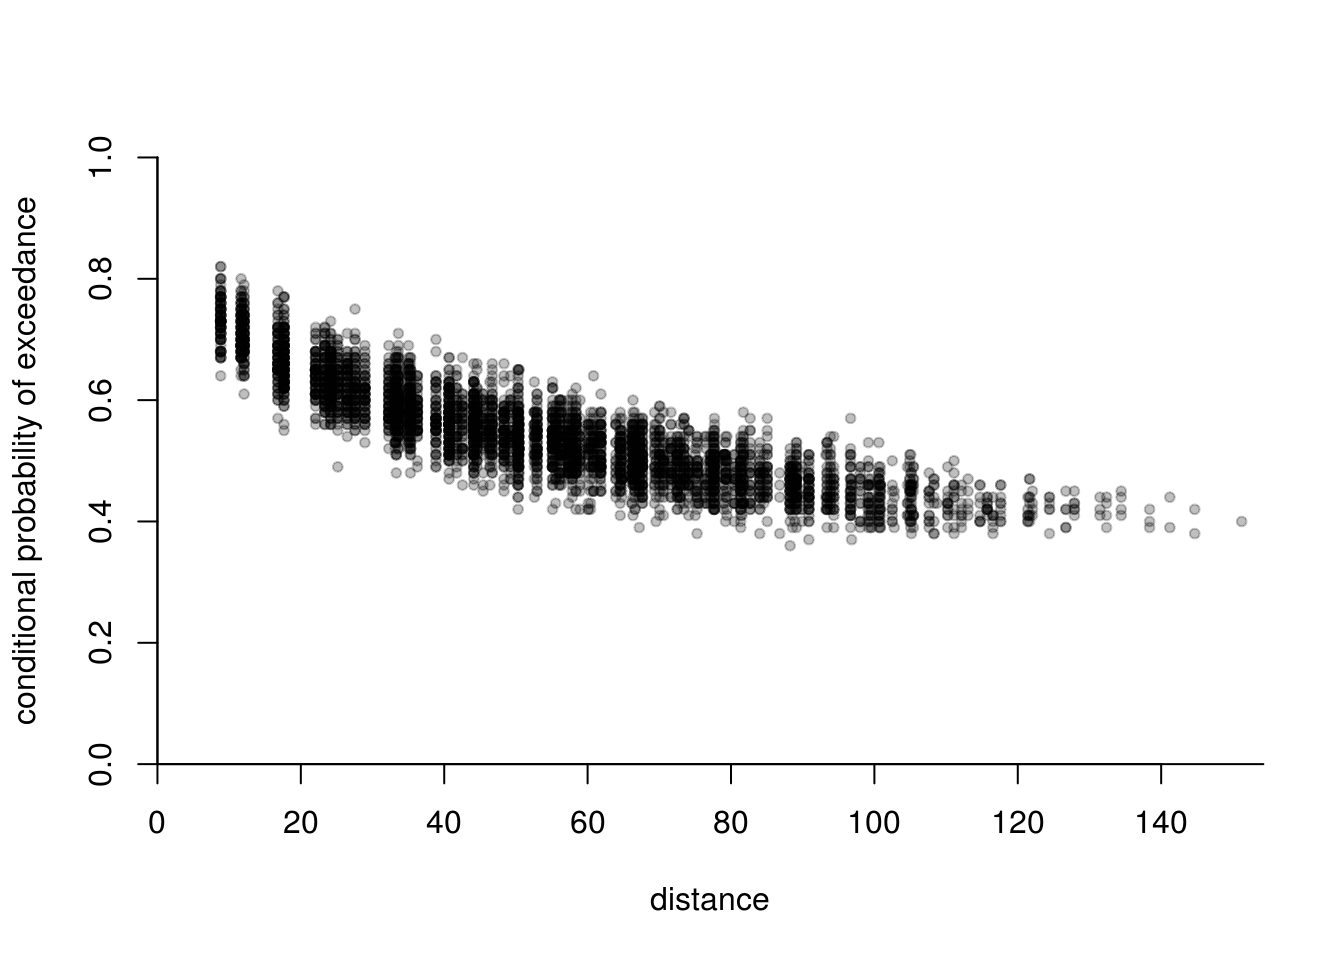
\includegraphics{mevtuto_files/figure-latex/fitvariocloud-1.pdf}

\begin{Shaded}
\begin{Highlighting}[]
 \CommentTok{# Constrained optimization}
 \CommentTok{# Minimize distance between extremal coefficient from fitted variogram}
\NormalTok{ mindistpvario <-}\StringTok{ }\ControlFlowTok{function}\NormalTok{(par, emp, coord)\{}
\NormalTok{ alpha <-}\StringTok{ }\NormalTok{par[}\DecValTok{1}\NormalTok{]; }\ControlFlowTok{if}\NormalTok{(}\OperatorTok{!}\KeywordTok{isTRUE}\NormalTok{(}\KeywordTok{all}\NormalTok{(alpha }\OperatorTok{>}\StringTok{ }\DecValTok{0}\NormalTok{, alpha }\OperatorTok{<}\StringTok{ }\DecValTok{2}\NormalTok{)))\{}\KeywordTok{return}\NormalTok{(}\FloatTok{1e10}\NormalTok{)\}}
\NormalTok{ scale <-}\StringTok{ }\NormalTok{par[}\DecValTok{2}\NormalTok{]; }\ControlFlowTok{if}\NormalTok{(scale }\OperatorTok{<=}\StringTok{ }\DecValTok{0}\NormalTok{)\{}\KeywordTok{return}\NormalTok{(}\FloatTok{1e10}\NormalTok{)\}}
\NormalTok{ a <-}\StringTok{ }\NormalTok{par[}\DecValTok{3}\NormalTok{]; }\ControlFlowTok{if}\NormalTok{(a}\OperatorTok{<}\DecValTok{1}\NormalTok{)\{}\KeywordTok{return}\NormalTok{(}\FloatTok{1e10}\NormalTok{)\}}
\NormalTok{ rho <-}\StringTok{ }\NormalTok{par[}\DecValTok{4}\NormalTok{]; }\ControlFlowTok{if}\NormalTok{(}\KeywordTok{abs}\NormalTok{(rho) }\OperatorTok{>=}\StringTok{ }\NormalTok{pi}\OperatorTok{/}\DecValTok{2}\NormalTok{)\{}\KeywordTok{return}\NormalTok{(}\FloatTok{1e10}\NormalTok{)\}}
\NormalTok{ semivariomat <-}\StringTok{ }\NormalTok{mgp}\OperatorTok{::}\KeywordTok{power.vario}\NormalTok{(}\KeywordTok{distg}\NormalTok{(coord, a, rho), }\DataTypeTok{alpha =}\NormalTok{ alpha, }\DataTypeTok{scale =}\NormalTok{ scale)}
   \KeywordTok{sum}\NormalTok{((}\DecValTok{2}\OperatorTok{*}\NormalTok{(}\DecValTok{1}\OperatorTok{-}\KeywordTok{pnorm}\NormalTok{(}\KeywordTok{sqrt}\NormalTok{(semivariomat[}\KeywordTok{lower.tri}\NormalTok{(semivariomat)]}\OperatorTok{/}\DecValTok{2}\NormalTok{))) }\OperatorTok{-}\StringTok{ }\NormalTok{emp)}\OperatorTok{^}\DecValTok{2}\NormalTok{)}
\NormalTok{ \}}
 \CommentTok{# constrained optimization for the parameters}
\NormalTok{ hin <-}\StringTok{ }\ControlFlowTok{function}\NormalTok{(par, ...)\{}
   \KeywordTok{c}\NormalTok{(}\FloatTok{1.99}\OperatorTok{-}\NormalTok{par[}\DecValTok{1}\NormalTok{], }\FloatTok{-1e-5} \OperatorTok{+}\StringTok{ }\NormalTok{par[}\DecValTok{1}\NormalTok{],}
     \FloatTok{-1e-5} \OperatorTok{+}\StringTok{ }\NormalTok{par[}\DecValTok{2}\NormalTok{],}
\NormalTok{     par[}\DecValTok{3}\NormalTok{]}\OperatorTok{-}\DecValTok{1}\NormalTok{,}
\NormalTok{     pi}\OperatorTok{/}\DecValTok{2} \OperatorTok{-}\StringTok{ }\NormalTok{par[}\DecValTok{4}\NormalTok{],}
\NormalTok{     par[}\DecValTok{4}\NormalTok{]}\OperatorTok{+}\NormalTok{pi}\OperatorTok{/}\DecValTok{2}\NormalTok{)}
\NormalTok{   \}}
\NormalTok{ opt <-}\StringTok{ }\NormalTok{alabama}\OperatorTok{::}\KeywordTok{auglag}\NormalTok{(}\DataTypeTok{par =} \KeywordTok{c}\NormalTok{(}\FloatTok{0.5}\NormalTok{, }\DecValTok{30}\NormalTok{, }\FloatTok{1.5}\NormalTok{, }\FloatTok{0.5}\NormalTok{),}
                        \DataTypeTok{hin =}\NormalTok{ hin, }\DataTypeTok{control.optim =} \KeywordTok{list}\NormalTok{(}\DataTypeTok{parscale =} \KeywordTok{c}\NormalTok{(}\FloatTok{0.5}\NormalTok{, }\DecValTok{30}\NormalTok{, }\FloatTok{1.5}\NormalTok{, }\FloatTok{0.5}\NormalTok{)),}
                         \DataTypeTok{fn =} \ControlFlowTok{function}\NormalTok{(par)\{}
                           \KeywordTok{mindistpvario}\NormalTok{(par, }\DataTypeTok{emp =}\NormalTok{ extdat[,}\StringTok{'prob'}\NormalTok{], }\DataTypeTok{coord =}\NormalTok{ coord)\})}
\end{Highlighting}
\end{Shaded}

\begin{verbatim}
## Min(hin):  0.49999 
## Outer iteration:  1 
## Min(hin):  0.49999 
## par:  0.5 30 1.5 0.5 
## fval =   77.37 
##  
## Outer iteration:  2 
## Min(hin):  0.3992261 
## par:  0.668296 74.8862 1.39923 0.556808 
## fval =   6.52 
##  
## Outer iteration:  3 
## Min(hin):  0.3992502 
## par:  0.668285 74.8855 1.39925 0.556807 
## fval =   6.52 
## 
\end{verbatim}

\begin{Shaded}
\begin{Highlighting}[]
 \KeywordTok{stopifnot}\NormalTok{(opt}\OperatorTok{$}\NormalTok{kkt1, opt}\OperatorTok{$}\NormalTok{kkt2)}
 \CommentTok{# Plotting the extremogram in the deformed space}
\NormalTok{ distfa <-}\StringTok{ }\KeywordTok{distg}\NormalTok{(}\DataTypeTok{loc =}\NormalTok{ coord, opt}\OperatorTok{$}\NormalTok{par[}\DecValTok{3}\NormalTok{], opt}\OperatorTok{$}\NormalTok{par[}\DecValTok{4}\NormalTok{])}
 \KeywordTok{plot}\NormalTok{(}\KeywordTok{c}\NormalTok{(distfa[}\KeywordTok{lower.tri}\NormalTok{(distfa)]), extdat[,}\DecValTok{2}\NormalTok{], }\DataTypeTok{pch =} \DecValTok{20}\NormalTok{,}
 \DataTypeTok{col =}\NormalTok{ scales}\OperatorTok{::}\KeywordTok{alpha}\NormalTok{(}\DecValTok{1}\NormalTok{,}\FloatTok{0.1}\NormalTok{), }\DataTypeTok{yaxs =} \StringTok{"i"}\NormalTok{, }\DataTypeTok{xaxs =} \StringTok{"i"}\NormalTok{, }\DataTypeTok{bty =} \StringTok{'l'}\NormalTok{,}
      \DataTypeTok{xlab =} \StringTok{"distance"}\NormalTok{, }\DataTypeTok{ylab=} \StringTok{"cond. prob. of exceedance"}\NormalTok{, }\DataTypeTok{ylim =} \KeywordTok{c}\NormalTok{(}\DecValTok{0}\NormalTok{,}\DecValTok{1}\NormalTok{))}
 \KeywordTok{lines}\NormalTok{(}\DataTypeTok{x =}\NormalTok{ (distvec <-}\StringTok{ }\KeywordTok{seq}\NormalTok{(}\DecValTok{0}\NormalTok{,}\DecValTok{200}\NormalTok{, }\DataTypeTok{length =} \DecValTok{1000}\NormalTok{)), }\DataTypeTok{col =} \DecValTok{2}\NormalTok{, }\DataTypeTok{lwd =} \DecValTok{2}\NormalTok{,}
       \DecValTok{2}\OperatorTok{*}\NormalTok{(}\DecValTok{1}\OperatorTok{-}\KeywordTok{pnorm}\NormalTok{(}\KeywordTok{sqrt}\NormalTok{(}\KeywordTok{power.vario}\NormalTok{(distvec, }\DataTypeTok{alpha =}\NormalTok{ opt}\OperatorTok{$}\NormalTok{par[}\DecValTok{1}\NormalTok{], }\DataTypeTok{scale =}\NormalTok{ opt}\OperatorTok{$}\NormalTok{par[}\DecValTok{2}\NormalTok{])}\OperatorTok{/}\DecValTok{2}\NormalTok{))))}
\end{Highlighting}
\end{Shaded}

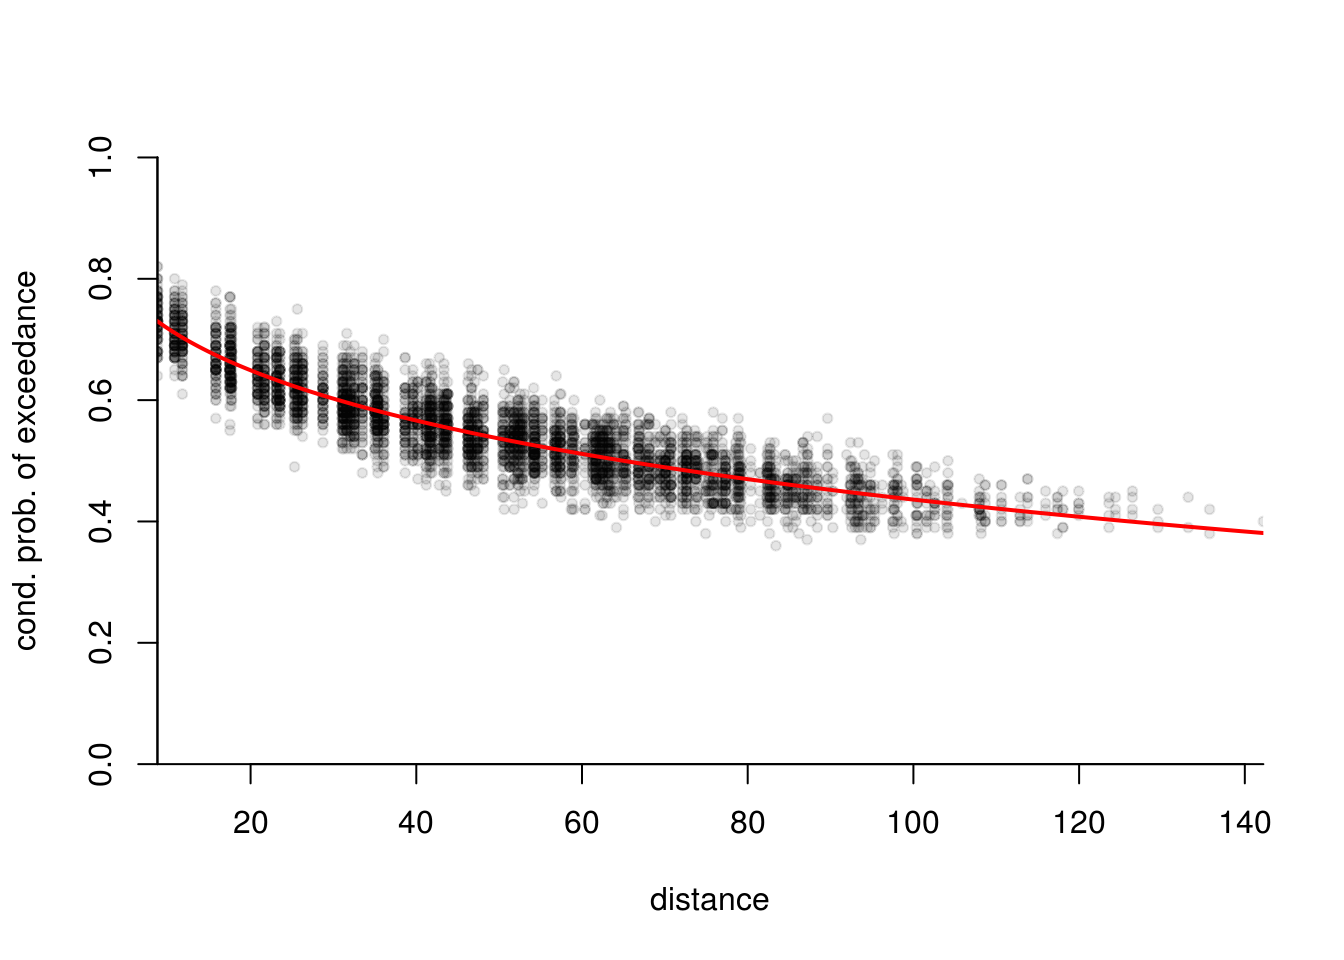
\includegraphics{mevtuto_files/figure-latex/fitvariocloud-2.pdf}

\bibliography{biblio.bib}


\end{document}
